\documentclass[journal,article,submit,pdftex,moreauthors]{Definitions/mdpi} 

\firstpage{1} 
\makeatletter 
\setcounter{page}{\@firstpage} 
\makeatother
\pubvolume{1}
\issuenum{1}
\articlenumber{0}
\pubyear{2025}
\copyrightyear{2025}
\datereceived{ } 
\daterevised{ }
\dateaccepted{ } 
\datepublished{ }
\hreflink{https://doi.org/}

\Title{Reconocimiento de Emociones Faciales en Tiempo Real para Adultos mediante Aplicación Móvil Android: Sistema Basado en CNN con Arquitectura de Microservicios para Contextos de Recursos Limitados}

\TitleCitation{Reconocimiento de Emociones Faciales en Tiempo Real para Adultos mediante Aplicación Móvil Android}

\newcommand{\orcidauthorA}{0000-0001-7725-8702}
\newcommand{\orcidauthorB}{0009-0008-7691-4542}
\newcommand{\orcidauthorC}{0009-0003-5637-2487}

\Author{Jhafet Martín Cánepa Maceda $^{1,}$*\orcidA{}, Christopher Antonio Pillihuamán Santiago $^{1}$\orcidB{} and Jorge Eduardo Castañeda Alban $^{1}$\orcidC{}}

\AuthorNames{Jhafet Martín Cánepa Maceda, Christopher Antonio Pillihuamán Santiago and Jorge Eduardo Castañeda Alban}

\AuthorCitation{Cánepa Maceda, J.M.; Pillihuamán Santiago, C.A.; Castañeda Alban, J.E.}

\address{%
	$^{1}$ \quad Universidad San Ignacio de Loyola, Facultad de Ingeniería, Programa de Ingeniería de Sistemas de Información, Av. La Fontana 550, La Molina, Lima 15024, Perú; jhafet.canepa@usil.pe (J.M.C.M.); c.pillihuaman@usil.pe (C.A.P.S.); jcastaneda@usil.edu.pe (J.E.C.A.)}

\corres{Correspondence: jcastaneda@usil.edu.pe; Tel.: +51-939-844-835}

\abstract{El reconocimiento de emociones faciales constituye una habilidad socioemocional fundamental para la interacción humana efectiva, cuyo déficit afecta significativamente la empleabilidad, relaciones interpersonales y calidad de vida de adultos entre 18-60 años. La detección tradicional de estas deficiencias requiere evaluaciones clínicas especializadas mediante instrumentos como el Reading the Mind in the Eyes Test, las cuales son costosas, consumen tiempo considerable y tienen accesibilidad limitada en contextos de recursos restringidos como regiones de Latinoamérica con infraestructura deficiente. Aunque métodos terapéuticos convencionales basados en tarjetas ilustradas estáticas han sido empleados durante décadas, estos carecen de retroalimentación objetiva cuantificable y generan limitada adherencia debido a su naturaleza no interactiva. Este estudio se centró en el análisis automatizado de expresiones faciales mediante técnicas de visión por computadora y desarrolló un sistema de Serious Game utilizando arquitecturas de redes neuronales convolucionales (CNN) para reconocimiento emocional en tiempo real. Utilizamos un modelo ensemble que combina EfficientNetB1, CNN personalizada de 5 capas convolucionales y análisis de 68 landmarks faciales mediante dlib, entrenado sobre el dataset FER2013 con 28,709 imágenes categorizadas en 5 emociones básicas (enojo, disgusto, neutral, feliz, triste). Implementamos una arquitectura de microservicios que integra backend en Go 1.21 (framework Gin) conectado a servicios especializados de Machine Learning en Python 3.11 (FastAPI), ejecutándose en servidor que se comunica con una aplicación móvil Android nativa desarrollada en Kotlin 1.9 con Android Studio, utilizando TensorFlow Lite 2.15 para inferencia on-device y OpenCV 4.8 para procesamiento de imágenes. El modelo desarrollado fue embebido en una aplicación smartphone Android que detecta emociones capturando y procesando expresiones faciales con una precisión promedio de 95.8\%, sensibilidad de 95.4\% y especificidad de 96.2\% en clasificación de las 5 emociones básicas (enojo, disgusto, neutral, feliz, triste) con tiempo de inferencia promedio de 187 milisegundos (rango: 34-820ms) por análisis completo en condiciones reales de uso.}

\keyword{Reconocimiento emocional facial; Aplicación móvil Android; Redes neuronales convolucionales; Serious Game; TensorFlow; OpenCV; Machine Learning; Adultos}

\usepackage{amssymb}

\begin{document}
	
	\section{Introducción}
	
	Una de las capacidades cognitivas fundamentales que afecta el desarrollo socioemocional y la integración social de adultos (18-60 años) universalmente es el reconocimiento de emociones faciales. El reconocimiento emocional facial ocurre cuando el sistema visual y cognitivo del cerebro procesa e interpreta correctamente las configuraciones musculares específicas del rostro humano que comunican estados emocionales \cite{ref11,ref12,ref33}. Esta habilidad es esencial para la teoría de la mente, permitiendo atribuir estados mentales, intenciones y emociones a otros individuos \cite{ref31}. Las deficiencias en reconocimiento emocional afectan aproximadamente al 15-20\% de la población adulta en diversos grados de severidad, manifestándose particularmente en condiciones del neurodesarrollo, trastornos del espectro autista y alexitimia \cite{ref7,ref9,ref13}.
	
	En diversos contextos clínicos y terapéuticos globalmente, el reconocimiento emocional es evaluado mediante técnicas psicométricas que requieren la participación de profesionales especializados certificados en neuropsicología o psicología clínica \cite{ref14,ref26,ref31}. Sin embargo, este enfoque tradicional es costoso, consume tiempo considerable, y resulta estresante para pacientes con déficits socioemocionales que requieren monitoreo frecuente \cite{ref26}. Este método tradicional puede introducir sesgos subjetivos del evaluador y limita la frecuencia de evaluaciones debido a restricciones presupuestarias \cite{ref18}.
	
	En regiones de recursos limitados, especialmente donde centros especializados, equipamiento tecnológico y personal capacitado son escasos, la inmovilidad de los métodos clínicos estándar genera considerables inconvenientes a pacientes que frecuentemente deben viajar distancias prolongadas para acceder a evaluaciones especializadas \cite{ref27}.
	
	Esto ha impulsado la necesidad de alternativas mejoradas a los métodos existentes de evaluación del reconocimiento emocional y consecuentemente la conducción de múltiples estudios para encontrar métodos automatizados mediante la comunidad científica en años recientes. Estudios previos han establecido que las expresiones emocionales pueden correlacionarse objetivamente con configuraciones específicas de acción muscular facial codificadas mediante el Facial Action Coding System (FACS) \cite{ref33,ref11,ref12,ref22}, regiones que contienen información visual densa analizable mediante técnicas de visión por computadora.
	
	Este estudio tuvo como objetivo desarrollar e implementar una aplicación smartphone que se enfoca en el análisis automatizado de expresiones faciales mediante técnicas de Deep Learning. Esta es una aplicación móvil multiplataforma Android que detecta emociones faciales mediante captura fotográfica y análisis en tiempo real (enfoque no invasivo). Proporciona acceso facilitado a entrenamiento en reconocimiento emocional principalmente para adultos en áreas remotas donde el acceso a profesionales especializados y tecnologías asistivas es limitado.
	
	Este estudio empleó una filosofía positivista. Esto se debe a que métodos cuantitativos, tales como análisis estadístico comparativo, son recomendados para investigar la relación cuantitativa entre precisión de modelos CNN y niveles de accuracy en reconocimiento emocional en población adulta \cite{ref8,ref15}. La investigación positivista proporciona resultados confiables, consistentes e imparciales \cite{ref8}.
	
	En este estudio, se desarrolló una aplicación móvil Android nativa que opera en sistema operativo Android mediante desarrollo en Kotlin 1.9 utilizando el Entorno de Desarrollo Integrado (IDE) Android Studio, empleando imágenes de expresiones faciales capturadas en tiempo real. Esta aplicación actúa como interfaz de usuario o frontend mediante la cual el usuario se comunica con nuestro Modelo de Detección de Emociones implementado con TensorFlow Lite. El usuario inicia la aplicación y utiliza la cámara del dispositivo para capturar fotografías del rostro. La imagen es transferida al servidor FastAPI, que ejecuta nuestro modelo de análisis CNN, mediante la conexión a internet del dispositivo. El procesamiento de imágenes se ejecuta en un servidor basado en Python 3.11 con framework FastAPI, mientras que la gestión de usuarios, autenticación y sesiones terapéuticas se maneja mediante backend desarrollado en Go 1.21 con framework Gin, garantizando arquitectura de microservicios escalable y eficiente.
	
	Los métodos convencionales de entrenamiento en reconocimiento emocional, basados predominantemente en tarjetas ilustradas estáticas presentadas por terapeutas, carecen de retroalimentación objetiva cuantificable y no generan métricas de progreso longitudinal que permitan ajustes terapéuticos basados en evidencia \cite{ref10,ref14,ref24}. La convergencia de avances recientes en arquitecturas de redes neuronales convolucionales específicamente optimizadas para dispositivos móviles como MobileNetV2 y EfficientNet \cite{ref3,ref20,ref21}, la madurez de frameworks de Machine Learning como TensorFlow y PyTorch \cite{ref6,ref7}, y la ubicuidad de smartphones Android de gama media ($\geq$6GB RAM) con capacidades de procesamiento on-device \cite{ref2,ref5}, han generado oportunidades sin precedentes para desarrollar sistemas de evaluación y entrenamiento emocional objetivos, escalables y accesibles.
	
	Los datasets públicos de referencia como CK+ (Extended Cohn-Kanade) con 593 secuencias de adultos 18-50 años \cite{ref14}, FER2013 con 35,887 imágenes etiquetadas en 7 emociones básicas \cite{ref16,ref17}, y AffectNet conteniendo 450,000 imágenes anotadas de expresiones in-the-wild \cite{ref13}, proporcionan recursos fundamentales para entrenar modelos CNN robustos. Arquitecturas recientes han alcanzado accuracy superiores al 95\% en datasets controlados, aunque el rendimiento en FER2013 típicamente se sitúa en 68-88\% debido a su naturaleza desafiante con variabilidad en iluminación, poses y oclusiones parciales \cite{ref3,ref9,ref19}.
	
	A pesar de estos avances tecnológicos, persisten brechas críticas: (1) el 89\% de estudios se concentra en población pediátrica dejando desatendida la población adulta donde las necesidades son igualmente apremiantes pero clínicamente distintas \cite{ref18}; (2) ningún estudio identificado aborda específicamente contextos latinoamericanos de recursos limitados con conectividad variable; (3) la mayoría describe prototipos sin validación clínica rigurosa o sistemas cloud-dependent que requieren conectividad constante \cite{ref1,ref2}.
	
	Este estudio aborda estas brechas mediante el desarrollo de un sistema de serious game específicamente diseñado para adultos de 18-60 años, implementando arquitectura offline-first que garantiza funcionalidad en contextos de conectividad intermitente mediante sincronización diferida, y validando el sistema mediante pruebas de campo en centros de atención de Lima y Tumbes, Perú, con población objetivo de 49 adultos diagnosticados con déficits en reconocimiento emocional. Las contribuciones específicas incluyen: (1) arquitectura técnica escalable integrando backend Go, servicios ML Python/FastAPI y aplicación Android Kotlin con persistencia MySQL y caché Redis; (2) modelo CNN ensemble optimizado alcanzando 95.8\% accuracy mediante combinación ponderada de EfficientNetB1, CNN personalizada y análisis de landmarks faciales sobre dataset FER2013; (3) validación técnica con 49 adultos en contextos de recursos limitados de Perú, demostrando precisión promedio de 80.2\% en reconocimiento emocional en condiciones reales de uso; (4) evidencia de satisfacción del 83.1\% entre usuarios y terapeutas en términos de facilidad de uso y funcionalidad del sistema.
	
	La estructura de este artículo es la siguiente: la Sección 2 revisa trabajos relacionados sobre aplicaciones móviles de reconocimiento emocional y serious games; la Sección 3 detalla la metodología del sistema incluyendo arquitectura técnica, diseño del modelo CNN y stack tecnológico; la Sección 4 presenta el diseño del estudio experimental; la Sección 5 expone resultados cuantitativos; la Sección 6 discute hallazgos y limitaciones; y la Sección 7 concluye con direcciones futuras de investigación.
	
	\section{Trabajos Relacionados}
	
	Esta sección analiza implementaciones técnicas previas de sistemas de reconocimiento emocional facial mediante Deep Learning, arquitecturas CNN optimizadas para dispositivos móviles, y aplicaciones Android para intervenciones socioemocionales, identificando brechas metodológicas críticas que esta investigación aborda.
	
	\subsection{Aplicaciones móviles Android para reconocimiento emocional facial}
	
	El desarrollo de aplicaciones móviles para reconocimiento de emociones faciales ha experimentado crecimiento exponencial en años recientes, impulsado por la madurez de frameworks como TensorFlow Lite y la disponibilidad de datasets públicos robustos. Alshamsi (2018) \cite{ref1} desarrolló Emotii, una aplicación Android para reconocimiento emocional multimodal (facial y vocal) desplegada en Google Play Store, implementando arquitectura cliente-servidor donde imágenes capturadas mediante cámara del dispositivo son transmitidas vía conexión de datos a servidor con modelo CNN en backend Python. El sistema alcanzó accuracy excepcional de 97.26\% sobre los datasets CK+ y RAVDESS, aunque la dependencia crítica de conectividad constante limitó su funcionalidad en regiones con infraestructura deficiente. Su estudio con 45 usuarios adultos demostró satisfacción del 89\% respecto a usabilidad de interfaz, pero identificó como limitación principal la latencia promedio de 3.2 segundos por análisis debido a transmisión de datos.
	
	Saumell (2018) \cite{ref2} implementó un sistema de detección emocional en tiempo real específicamente optimizado para Android mediante desarrollo en Java utilizando Android Studio, ejecutándose completamente on-device en smartphone Nexus 5 con procesador Snapdragon 800. Su arquitectura integra OpenCV 3.4 para captura de frames de cámara frontal a 15 FPS, preprocesamiento mediante detección facial Haar Cascades, y clasificación mediante SVM entrenado sobre dataset Radboud Faces con 8 emociones. Los resultados experimentales demostraron accuracy de 87-94\% dependiendo de condiciones de iluminación, con latencia promedio de 67ms por frame, estableciendo viabilidad técnica de procesamiento completamente local. Sin embargo, el uso de SVM en lugar de arquitecturas CNN modernas limitó la precisión comparada con aproximaciones basadas en Deep Learning.
	
	Zhu et al. (2024) \cite{ref3} desarrollaron I-MobileNetV2, una arquitectura CNN específicamente optimizada para reconocimiento emocional en smartphones mediante integración de módulos Squeeze-and-Excitation (SE) attention que incrementan la sensibilidad a características discriminativas mientras mantienen eficiencia computacional. Su implementación en smartphone Huawei P60 con procesador Kirin 9000s (6GB RAM) alcanzó accuracy de 95.96\% sobre CK+ y 68.62\% sobre FER2013 con solo 3.26M parámetros (reducción de 83.8\% versus MobileNetV2 estándar), demostrando tiempo de inferencia de 42ms por imagen mediante TensorFlow Lite con cuantización INT8. Este trabajo establece que arquitecturas con attention mechanisms representan el estado del arte actual para aplicaciones móviles, aunque no reportan validación clínica con usuarios reales ni evaluación en condiciones in-the-wild variables.
	
	\subsection{Arquitecturas CNN y técnicas de Deep Learning para clasificación emocional}
	
	El reconocimiento automático de expresiones faciales mediante redes neuronales convolucionales ha alcanzado niveles de precisión cercanos o superiores a capacidad humana en datasets controlados. Debnath et al. (2022) \cite{ref9} implementaron una arquitectura CNN compacta de 4 capas convolucionales entrenada sobre FER2013, alcanzando validation accuracy de 91.01\% mediante técnicas de data augmentation (rotación $\pm$25°, flip horizontal, brightness adjustment $\pm$20\%, zoom $\pm$10\%) y dropout de 0.5 para prevenir overfitting. Su análisis exhaustivo de matrices de confusión reveló que las emociones ``miedo'' y ``sorpresa'' presentaban mayor tasa de confusión mutua (31.2\% de clasificaciones erróneas), consistente con similitudes anatómicas en configuración facial de ambas expresiones según el Facial Action Coding System \cite{ref33,ref11,ref12}. Críticamente, su estudio demostró que la diversidad del dataset de entrenamiento impacta significativamente el desempeño: modelos entrenados exclusivamente en FER2013 presentaron accuracy 12.8\% inferior cuando evaluados sobre CK+ comparado con modelos entrenados en datasets combinados.
	
	Agung et al. (2024) \cite{ref7} realizaron estudio comparativo exhaustivo de arquitecturas mediante transfer learning, evaluando Inception-V3, MobileNet-V2, ResNet50 y VGG16 sobre el dataset Emognition (2,414 imágenes faciales con anotaciones multimodales). Los resultados demostraron que Inception-V3 alcanzó accuracy óptima de 96\% tras fine-tuning de últimas 10 capas con learning rate 0.0001, mientras MobileNet-V2 logró 89\% con ventaja crítica de requerir solo 3.4M parámetros versus 23.8M de Inception-V3, estableciendo trade-off fundamental accuracy-eficiencia para aplicaciones móviles. Su validación cruzada externa sobre datasets JAFFE y KDEF confirmó capacidad de generalización con degradación controlada de accuracy (4.2\% y 6.7\% respectivamente), evidenciando robustez del transfer learning desde ImageNet.
	
	Elsheikh et al. (2024) \cite{ref8} propusieron arquitectura innovadora AA-DCN (Anti-Aliased Deep Convolutional Network) que integra filtros anti-aliasing entre capas de pooling para preservar información espacial de alta frecuencia crítica para reconocimiento de micro-expresiones faciales. Su modelo alcanzó accuracy excepcional de 99.26\% sobre CK+, 96.84\% sobre JAFFE, y 88.12\% sobre RAF-DB mediante entrenamiento con Adam optimizer (lr=0.001, beta1=0.9, beta2=0.999), batch size 32, y 150 épocas con early stopping (patience=15). Análisis de mapas de activación mediante Grad-CAM revelaron que el modelo enfoca atención en regiones periorbitales (41\% de activación) y bucales (37\%), consistente con teorías psicológicas sobre expresividad emocional \cite{ref11,ref12}.
	
	Qian et al. (2025) \cite{ref10} condujeron estudio benchmark comparando 10 arquitecturas CNN (VGG16, VGG19, ResNet50, ResNet101, DenseNet, GoogLeNet V1, MobileNet V1, EfficientNet V2, ShuffleNet V2, RepVGG) sobre FER2013 mediante protocolo estandarizado (split 80/10/10, data augmentation, 100 épocas). Los resultados establecieron que EfficientNet V2 alcanzó el mejor balance accuracy-eficiencia con 68.7\% accuracy, seguido por ResNet50 y ResNet101 con 68.1\% accuracy. Este estudio proporciona evidencia empírica robusta para selección de arquitecturas en aplicaciones móviles con restricciones computacionales, destacando los trade-offs entre precisión y eficiencia computacional.
	
	\subsection{Implementaciones Android con TensorFlow Lite y OpenCV}
	
	La convergencia de TensorFlow Lite para inferencia on-device y OpenCV para procesamiento de imágenes ha habilitado implementaciones Android completamente funcionales sin dependencia de conectividad. El repositorio GitHub lampadovnikita \cite{ref6} documenta implementación completa en Kotlin de aplicación Android para reconocimiento emocional utilizando TensorFlow Lite 2.x y ML Kit de Google para detección facial, entrenada sobre dataset híbrido combinando CK+, JAFFE, FER2013 y RAF-DB (46,614 imágenes totales). La arquitectura implementa pipeline: (1) captura de frame mediante Camera2 API, (2) detección facial mediante ML Kit con tiempo promedio 12ms, (3) preprocesamiento (conversión a escala de grises, resize a 48$\times$48px, normalización [0,1]), (4) inferencia mediante modelo TFLite cuantizado INT8 con latencia 28ms en Snapdragon 665. El código fuente abierto bajo licencia MIT constituye referencia técnica valiosa para desarrolladores, aunque no reporta validación clínica ni métricas de accuracy sobre datasets estándar.
	
	Haq et al. (2024) \cite{ref5} desarrollaron sistema de reconocimiento emocional en tiempo real optimizado mediante MobileNet-V1 con modificaciones arquitectónicas: incremento de filtros en capas convolucionales finales (512$\rightarrow$1024), adición de capa Global Average Pooling, y dos capas Dense con dropout 0.5. Su implementación Android mediante TensorFlow Lite alcanzó accuracy de 97.9\% sobre FER2013 tras 80 épocas de entrenamiento con data augmentation agresivo (ShearRange=0.2, ZoomRange=0.2, horizontal\_flip=True), SGD optimizer con momentum 0.9 y learning rate scheduling (decay factor 0.5 cada 20 épocas). La evaluación en smartphone Samsung Galaxy A52 (Snapdragon 720G, 6GB RAM) demostró procesamiento de 18.3 FPS con consumo energético de 421mW, estableciendo viabilidad de operación continua durante sesiones terapéuticas prolongadas.
	
	Nan et al. (2022) \cite{ref4} propusieron A-MobileNet, arquitectura que integra módulos attention en bloques invertidos residuales de MobileNetV2 para incrementar sensibilidad a características discriminativas faciales. Su implementación alcanzó accuracy de 88.11\% sobre RAF-DB (dataset in-the-wild particularmente desafiante) y 91.23\% sobre FERPlus mediante entrenamiento en dos fases: (1) preentrenamiento en FER2013 durante 50 épocas, (2) fine-tuning en RAF-DB durante 30 épocas con learning rate reducido 10$\times$. Análisis de ablation studies demostraron que los módulos attention contribuyen +4.7\% accuracy absoluto, mientras separable convolutions reducen parámetros en 8.3$\times$ versus arquitecturas CNN estándar, confirmando efectividad del diseño.
	
	\subsection{Datasets públicos para entrenamiento de modelos emocionales}
	
	La disponibilidad de datasets públicos robustos ha sido crítica para avances en reconocimiento emocional mediante Deep Learning. Mollahosseini et al. (2017) \cite{ref13} desarrollaron AffectNet, el dataset in-the-wild de mayor escala conteniendo 450,000 imágenes faciales anotadas manualmente, recolectadas mediante queries en motores de búsqueda con términos emocionales en múltiples idiomas. El dataset incluye anotaciones de 8 emociones discretas (neutral, felicidad, tristeza, sorpresa, miedo, disgusto, enojo, desprecio), valencia continua [-10,+10] y arousal [0,10], con población diversa (edad promedio 33.2$\pm$12.4 años, 58\% mujeres, 42\% hombres, representación multi-étnica). Los modelos baseline reportados alcanzan accuracy de 58-65\% en clasificación de 8 emociones, estableciendo benchmark desafiante que refleja complejidad de expresiones naturales con variabilidad en iluminación, pose ($\pm$90°), oclusiones parciales y resoluciones heterogéneas (28$\times$28 a 800$\times$600px).
	
	Lucey et al. (2010) \cite{ref14} desarrollaron el Extended Cohn-Kanade Dataset (CK+), gold standard para evaluación de sistemas de reconocimiento emocional, conteniendo 593 secuencias de video de 123 participantes adultos (edad 18-50 años, media 25.3$\pm$7.8) con anotaciones FACS (Facial Action Coding System) y etiquetas de emoción validadas. Cada secuencia captura transición desde expresión neutral hasta emoción pico en condiciones controladas (iluminación uniforme, fondo negro, cámara frontal), con 327 secuencias etiquetadas en 7 emociones básicas. Los sistemas CNN modernos alcanzan accuracy superiores a 98\% sobre CK+, aunque esta precisión excepcional no generaliza a contextos in-the-wild debido a condiciones de captura idealizadas.
	
	Li \& Deng (2019) \cite{ref15} desarrollaron RAF-DB (Real-world Affective Faces Database), dataset específicamente diseñado para evaluar robustez en condiciones naturales mediante 30,000 imágenes faciales diversas recolectadas desde Flickr y búsquedas web, anotadas mediante crowdsourcing con 40 trabajadores independientes por imagen. El dataset implementa mecanismo de confiabilidad basado en concordancia inter-anotador, resultando en 15,339 imágenes básicas con alta confianza y 14,661 imágenes compuestas con emociones mixtas. Los estudios reportan que modelos entrenados exclusivamente en datasets controlados (CK+) experimentan degradación de accuracy de 15-22\% cuando evaluados sobre RAF-DB, evidenciando gap crítico entre laboratorio y aplicaciones reales.
	
	Goodfellow et al. (2015) \cite{ref16} introdujeron FER2013 mediante competición Kaggle, conteniendo 35,887 imágenes en escala de grises (48$\times$48px) extraídas automáticamente desde Google Image Search, categorizadas en 7 emociones mediante votación mayoritaria de múltiples anotadores. A pesar de limitaciones inherentes (baja resolución, ruido de anotación estimado 15-20\%, desbalance de clases), FER2013 ha emergido como benchmark estándar de la comunidad científica con 2,800+ citaciones, permitiendo comparación directa entre aproximaciones metodológicas. Los sistemas state-of-the-art alcanzan accuracy de 71-78\% mediante ensemble de modelos CNN con data augmentation exhaustivo, siendo Khaireddin y Chen (2021) \cite{ref17} quienes reportaron rendimiento destacado en este dataset desafiante.
	
	\subsection{Serious Games y gamificación para intervenciones terapéuticas}
	
	Los Serious Games constituyen aplicaciones digitales que integran mecánicas lúdicas con objetivos terapéuticos o educativos específicos, incrementando motivación intrínseca y adherencia mediante elementos de gamificación mientras mantienen rigor clínico \cite{ref24,ref26}. Vermeir et al. (2020) \cite{ref24} condujeron revisión sistemática con meta-análisis evaluando efectos de gamificación en entrenamiento cognitivo computarizado, analizando 31 estudios controlados aleatorios (N=2,486 participantes). Los resultados demostraron que intervenciones gamificadas producen tamaños de efecto significativamente superiores versus versiones no-gamificadas para outcomes cognitivos (d=0.37, IC 95\%: 0.21-0.53, p$<$0.001) y adherencia terapéutica (OR=2.14, IC 95\%: 1.67-2.74, p$<$0.001), aunque los autores advierten sobre heterogeneidad metodológica sustancial entre estudios.
	
	Matsouliadis et al. (2025) \cite{ref23} realizaron revisión sistemática de literatura sobre Speech Emotion Recognition en serious games, analizando 47 publicaciones (2015-2024) que integran reconocimiento multimodal (facial, vocal, fisiológico) en aplicaciones terapéuticas. Su análisis identificó que sistemas multimodales alcanzan accuracy promedio 13.2\% superior versus unimodales (facial solamente), aunque con trade-off de incrementar latencia de procesamiento 2.4$\times$ y complejidad de implementación. Críticamente, solo 19\% de estudios reportaron validación clínica rigurosa con grupo control, evidenciando brecha entre desarrollo técnico y evidencia empírica de efectividad terapéutica.
	
	Koptyra et al. (2024) \cite{ref25} propusieron framework para integración de reconocimiento emocional en pruebas de usabilidad de aplicaciones web, implementando captura facial mediante webcam sincronizada con interacciones del usuario (clicks, scroll, tiempo en tarea). Su estudio con 85 participantes demostró que eventos de usabilidad negativos (errores de navegación, formularios confusos) correlacionan significativamente con expresiones de frustración detectadas automáticamente (r=0.67, p$<$0.001), estableciendo viabilidad de métricas afectivas objetivas como complemento a cuestionarios subjetivos tradicionales.
	
	\subsection{Contexto de recursos limitados y adaptación cultural}
	
	La implementación de tecnologías asistivas en contextos de recursos limitados enfrenta desafíos únicos relacionados con infraestructura deficiente, disponibilidad de dispositivos, y adaptación cultural. Estudios previos documentan que en regiones rurales de Latinoamérica, aproximadamente 60\% de centros de atención carecen de conectividad estable a internet \cite{ref27,ref28}, mientras que 78\% de terapeutas no ha recibido capacitación formal en tecnologías digitales terapéuticas \cite{ref27}. Estas barreras estructurales demandan arquitecturas offline-first que garanticen funcionalidad independiente de conectividad, contrario a sistemas cloud-dependent prevalentes en literatura como los implementados por Alshamsi \cite{ref1}.
	
	No se identificaron publicaciones en bases indexadas (Scopus, Web of Science, IEEE Xplore) que aborden específicamente implementaciones técnicas de sistemas Machine Learning para reconocimiento emocional en adultos validadas en contextos latinoamericanos de recursos limitados, evidenciando vacío crítico en literatura científica.
	
	\subsection{Brechas identificadas y posicionamiento de esta investigación}
	
	El análisis sistemático de trabajos relacionados revela cinco brechas metodológicas fundamentales que esta investigación aborda:
	
	\begin{table}[H]
		\caption{Comparación de características técnicas y metodológicas con trabajos relacionados.\label{tab1}}
		\small
		\begin{adjustwidth}{-\extralength}{0cm}
			\begin{tabularx}{\fulllength}{lCCCCCC}
				\toprule
				\textbf{Estudio} & \textbf{Año} & \textbf{Población} & \textbf{N} & \textbf{Arquitectura CNN} & \textbf{Dataset} & \textbf{Conectividad} \\
				\midrule
				Saumell \cite{ref2} & 2018 & Adultos & - & SVM + Haar & Radboud & Offline \\
				Alshamsi \cite{ref1} & 2018 & Adultos & 45 & CNN + LSTM & CK+, RAVDESS & Requiere \\
				Debnath et al. \cite{ref9} & 2022 & General & - & CNN 4-layer & FER2013 & N/A \\
				Nan et al. \cite{ref4} & 2022 & General & - & A-MobileNet & RAF-DB & N/A \\
				Agung et al. \cite{ref7} & 2024 & Adultos & - & Inception-V3 & Emognition & N/A \\
				Zhu et al. \cite{ref3} & 2024 & General & - & I-MobileNetV2 & FER2013, CK+ & Offline \\
				Haq et al. \cite{ref5} & 2024 & General & - & MobileNet-V1 & FER2013 & Offline \\
				Elsheikh et al. \cite{ref8} & 2024 & Adultos 18-50 & - & AA-DCN & CK+, JAFFE & N/A \\
				\textbf{Este estudio} & \textbf{2025} & \textbf{Adultos 18-60} & \textbf{49} & \textbf{CNN ensemble} & \textbf{FER2013} & \textbf{Offline} \\
				\bottomrule
			\end{tabularx}
		\end{adjustwidth}
	\end{table}

	\textbf{Brecha 1 - Población objetivo adulta:} El análisis de 30 estudios recientes (2018-2025) revela que 87\% se enfoca en población pediátrica ($\leq$18 años) o población general sin especificación etaria. Solo 4 estudios \cite{ref1,ref2,ref7,ref8} abordan explícitamente población adulta, y ninguno implementa validación clínica rigurosa con grupo control en este segmento poblacional específico, a pesar de que déficits en reconocimiento emocional persisten en edad adulta con impactos significativos en empleabilidad y autonomía funcional \cite{ref7,ref13}.
	
	\textbf{Brecha 2 - Arquitectura offline-first:} El 73\% de implementaciones móviles identificadas requieren conectividad constante para transmisión de imágenes a servidores remotos con procesamiento cloud \cite{ref1}. Solo 27\% implementa inferencia on-device mediante TensorFlow Lite \cite{ref2,ref3,ref5,ref6}, pero ninguno documenta estrategias de sincronización diferida, gestión de caché distribuido, o mecanismos de degradación graceful para garantizar funcionalidad robusta en contextos de conectividad intermitente característicos de regiones de recursos limitados.
	
	\textbf{Brecha 3 - Validación clínica rigurosa:} Únicamente 17\% (5/30) de estudios analizados implementa diseños cuasiexperimentales o experimentales con grupo control que permitan establecer causalidad entre intervención y outcomes terapéuticos. El 83\% restante reporta: (a) validaciones técnicas sin participantes reales (47\%), (b) estudios de satisfacción de usuarios sin mediciones de efectividad clínica (23\%), o (c) diseños pre-post sin grupo control que no permiten descartar efectos de maduración o regresión a la media (13\%). Esta limitación crítica impide establecer evidencia empírica robusta sobre efectividad terapéutica real de tecnologías AI en contextos clínicos.
	
	\textbf{Brecha 4 - Contexto geográfico:} Ningún estudio identificado en búsquedas sistemáticas aborda específicamente implementación y validación en contextos latinoamericanos de recursos limitados con características distintivas: (a) conectividad $<$60\% de centros de atención \cite{ref28}, (b) dispositivos predominantemente de gama media ($\leq$6GB RAM, procesadores Snapdragon 6xx), (c) escasez crítica de profesionales especializados (solo 20\% de centros cuenta con personal capacitado en tecnologías asistivas \cite{ref27}), y (d) barreras geográficas con tiempos de traslado prolongados en regiones rurales. La concentración de investigación en países desarrollados (EE.UU., Reino Unido, China) limita aplicabilidad directa de hallazgos a contextos de infraestructura deficiente.
	
	\textbf{Brecha 5 - Documentación técnica completa:} Ningún trabajo analizado documenta exhaustivamente arquitectura de microservicios implementada, incluyendo: (a) stack tecnológico específico con versiones (backend framework, ORM, sistema de caché), (b) métricas cuantitativas de desempeño (latencia p50/p95/p99, throughput, consumo de memoria), (c) estrategias de escalabilidad horizontal, (d) mecanismos de manejo de errores y recuperación ante fallos, y (e) código fuente verificable en repositorios públicos. Esta carencia limita severamente reproducibilidad y transferencia tecnológica a otros contextos de investigación o implementación clínica.
	
	Esta investigación posiciona el sistema Serious Game como la primera implementación documentada que aborda simultáneamente estas cinco brechas críticas mediante: (1) enfoque específico en adultos 18-60 años con validación en campo real, (2) arquitectura offline-first con microservicios Go/Python y sincronización diferida mediante Redis, (3) validación técnica con 49 participantes adultos (79 sesiones totales) en centros de atención de Lima y Tumbes, recolectando métricas objetivas de precisión en reconocimiento emocional mediante la aplicación móvil, (4) adaptación contextual específica a limitaciones de infraestructura de regiones peruanas mediante co-diseño con terapeutas locales, y (5) documentación técnica exhaustiva de arquitectura, stack tecnológico, y métricas de desempeño que facilita reproducibilidad y transferencia tecnológica a contextos similares de recursos limitados en Latinoamérica.
	
	\section{Metodología}
	
	Este estudio se estructuró en tres fases principales: (1) diseño de la arquitectura tecnológica del sistema Serious Game con modelo CNN, (2) recolección y preprocesamiento del dataset de entrenamiento, y (3) validación clínica mediante diseño cuasiexperimental con análisis estadístico comparativo. La metodología integra desarrollo técnico de Machine Learning con evaluación rigurosa de efectividad terapéutica en adultos con déficits en reconocimiento emocional.
	
	\subsection{Método de recolección de datos}
	
	Para entrenar el modelo CNN de reconocimiento emocional, se utilizó el dataset público FER2013 \cite{ref16,ref17}, seleccionado por ser el benchmark estándar más ampliamente adoptado en investigación de expresiones faciales. El dataset contiene 35,887 imágenes en escala de grises (48$\times$48 píxeles) extraídas automáticamente mediante Google Image Search, categorizadas en 7 emociones básicas: Angry, Disgust, Fear, Happy, Neutral, Sad, Surprise. Las imágenes fueron anotadas mediante votación mayoritaria de múltiples evaluadores humanos independientes. El dataset se distribuyó en tres particiones: 28,709 imágenes para entrenamiento (80\%), 3,589 para validación (10\%), y 3,589 para evaluación final (10\%).
	
	Se desarrolló un pipeline automatizado de preprocesamiento para incrementar calidad y diversidad del dataset. Personal entrenado en visión por computadora implementó el sistema de procesamiento utilizando OpenCV 4.8 y Python 3.11, ejecutándose en servidor Linux Ubuntu 22.04 LTS. El preprocesamiento siguió cinco etapas secuenciales documentadas mediante scripts reproducibles en repositorio GitHub del proyecto.
	
	Con respecto al procesamiento de imágenes faciales, se aplicó técnica CLAHE (Contrast Limited Adaptive Histogram Equalization) con clip limit 2.0 para normalizar iluminación mediante ecualización adaptativa, técnica ampliamente utilizada en sistemas de reconocimiento emocional facial \cite{ref34,ref35}. Para minimizar efectos de variabilidad extrema en condiciones de captura que podrían afectar desempeño del modelo, esta técnica ecualizó histogramas localmente en regiones de 8$\times$8 píxeles. Este método fue fundamental para homogeneizar el dataset considerando que imágenes in-the-wild presentan heterogeneidad sustancial en condiciones de iluminación.
	
	Adicionalmente, se aplicó data augmentation durante entrenamiento para incrementar tamaño efectivo del dataset y prevenir overfitting. Las transformaciones aplicadas fueron: rotación aleatoria $\pm$15° (simula variaciones naturales de inclinación cefálica), flip horizontal con 50\% de probabilidad (duplica efectivamente ejemplos de entrenamiento), zoom aleatorio $\pm$10\% (simula variaciones de distancia focal entre cámara y rostro), y desplazamiento horizontal/vertical aleatorio $\pm$5\% (simula descentramiento facial en encuadre). Estas técnicas incrementaron el dataset efectivo de 28,709 a aproximadamente 115,000 ejemplos únicos por época de entrenamiento.
	
	Las características del dataset preprocesado se extrajeron mediante arquitectura CNN EfficientNetB1 \cite{ref21} pre-entrenada en ImageNet, utilizando transfer learning para aprovechar features de bajo nivel previamente aprendidas. El modelo base con 7.8M parámetros fue inicializado con pesos pre-entrenados, utilizando transfer learning para aprovechar features de bajo nivel previamente aprendidas. El modelo base con 5.3M parámetros fue inicializado con pesos pre-entrenados, y se agregaron capas superiores personalizadas: GlobalAveragePooling2D seguido de capa Dense con 512 neuronas y activación ReLU, Dropout con probabilidad 0.5 para regularización, y capa final Dense con 7 neuronas y activación Softmax para clasificación multiclase. El dataset preprocesado con estas características alimentó el entrenamiento del modelo durante 50 épocas con batch size 32.
	
	\subsection{Arquitectura del sistema}
	
	El diagrama arquitectónico de la Figura~\ref{fig1} muestra los componentes principales que integran el sistema de reconocimiento emocional Serious Game. El sistema propuesto para detección de emociones faciales consiste en cuatro módulos especializados: módulo de captura de imágenes, módulo de preprocesamiento y detección facial, módulo de clasificación emocional basado en CNN, y módulo de gestión de datos históricos. El sistema comprende dos componentes principales integrados mediante APIs RESTful: Frontend móvil y Backend distribuido, junto con algoritmos específicos de Machine Learning.
	
	\textbf{Stack Tecnológico Implementado:}
	
	El sistema integra tres componentes principales mediante arquitectura de microservicios:
	
	\textbf{Backend de Gestión de Usuarios (Go 1.21):} Desarrollado con framework Gin, implementa autenticación JWT con renovación automática, control de acceso basado en roles (admin, terapeuta, responsable), gestión de sesiones terapéuticas, y sistema de calificaciones con reasignación automática de terapeutas. Integra MySQL 8.0 para persistencia relacional y Redis 7.2 para cache distribuido y rate limiting diferenciado por rol. El backend expone APIs REST seguras con validación de tokens en cada request.
	
	\textbf{Servicio de Machine Learning (Python 3.11):} Implementado con FastAPI, ejecuta inferencia del modelo CNN mediante TensorFlow 2.15. Procesa imágenes faciales mediante OpenCV 4.8 y Pillow para preprocesamiento, aplica CLAHE para normalización de contraste, y genera predicciones con tiempos de respuesta $<$200ms por análisis. Implementa rate limiting mediante Redis con límites diferenciados: 100 análisis/día para terapeutas y responsables, sin límites para administradores. El servicio mantiene cache de sesiones con TTL de 2 horas y monitoreo automático de calidad de predicciones.
	
	\textbf{Aplicación Android (Kotlin 1.9):} Desarrollada con Jetpack Compose y Material Design 3, implementa arquitectura MVVM con Repository Pattern. Utiliza Retrofit 2.9.0 para comunicación HTTP con backends, Glide 4.16.0 para gestión eficiente de imágenes, y Security Crypto para encriptación local de datos sensibles. La aplicación soporta autenticación biométrica (huella dactilar/reconocimiento facial), captura de imágenes mediante cámara frontal o selección desde galería, y visualización de resultados históricos con gráficos interactivos. Mínimo SDK 30 (Android 11), target SDK 34.
	
	\begin{figure}[H]
		
\includegraphics[width=\textwidth]{fig1.png}
		\caption{Arquitectura propuesta del sistema de microservicios.\label{fig1}}
	\end{figure}
	
	\subsubsection{Frontend}
	
	El frontend es una aplicación móvil Android nativa desarrollada en Kotlin 1.9 con Android Studio que se conecta a servicios backend donde residen los módulos de detección, predicción y gestión de datos. La aplicación permite a usuarios capturar fotografías faciales mediante cámara frontal del dispositivo o seleccionar imágenes existentes en galería para envío al servidor de procesamiento. La app también despliega resultados del análisis emocional al usuario y facilita comunicación bidireccional con el módulo de gestión de datos mediante protocolo HTTPS con autenticación JWT.
	
	\subsubsection{Backend}
	
	El backend está compuesto por el módulo de detección facial, módulo de clasificación emocional CNN y módulo de gestión de datos, implementados como microservicios independientes. El módulo de detección facial garantiza identificación y extracción de región de interés (ROI) del rostro en fotografías enviadas, transmitiendo datos validados al módulo de clasificación. El módulo de clasificación emocional ejecuta inferencia del modelo CNN mediante TensorFlow Lite para generar predicciones de las 7 emociones básicas con sus respectivos niveles de confianza.
	
	El módulo de gestión de datos maneja cuentas de usuario, historiales de sesiones terapéuticas y resultados asociados a cada paciente. Se utilizó base de datos MySQL 8.0 para persistencia relacional y sistema de caché distribuido Redis 7.2 para optimización de desempeño y funcionalidad offline.
	
	\subsubsection{Métodos operacionales}
	
	En este estudio utilizamos Redes Neuronales Convolucionales con arquitectura EfficientNetB1, técnicas de transfer learning, preprocesamiento mediante OpenCV, y deployment en aplicación smartphone hospedada en servidor FastAPI. El diagrama de flujo en Figura~\ref{fig2} ilustra cómo opera el sistema propuesto.
	
	\begin{figure}[H]
		
\includegraphics[width=\textwidth]{fig2.png}
		\caption{Diagrama de flujo del proceso de reconocimiento emocional.\label{fig2}}
	\end{figure}
	
	Una aplicación móvil Android nativa que opera en sistema operativo Android fue desarrollada en Kotlin 1.9 utilizando el Entorno de Desarrollo Integrado (IDE) Android Studio. Esta aplicación actúa como interfaz de usuario o frontend mediante el cual el usuario se comunica con el Modelo de Detección de Emociones. El usuario inicia la aplicación y utiliza la cámara del dispositivo para capturar fotografías del rostro. La imagen es transferida al servidor FastAPI que ejecuta el modelo de análisis CNN mediante la conexión a internet del dispositivo. El procesamiento de imágenes ocurre en un servidor basado en Python 3.11 con framework FastAPI para servicios de Machine Learning, mientras que gestión de usuarios, autenticación y sesiones terapéuticas se maneja mediante backend desarrollado en Go 1.21 con framework Gin.
	
	\textbf{Fase 1. Extracción de la Región de Interés}
	
	El rostro completo constituye la ROI crítica para análisis emocional. Para obtener el ROI facial, primero se determina si existe un rostro detectable en la fotografía proporcionada. Esto se logra comparando cada imagen capturada contra un modelo de detección facial entrenado implementado mediante Haar Cascade de OpenCV \cite{ref32}. Una vez identificado el rostro, se extrae mediante bounding box rectangular con margen adicional del 20\% para incluir contexto periférico relevante (orejas, contorno facial), generando imagen recortada que se utiliza como entrada real para el procesamiento subsecuente.
	
	La extracción facial se logra mediante tres pasos automatizados secuenciales que garantizan calidad de la ROI:
	
	\textit{1. Localización del centro facial}
	
	Para detectar precisamente la región facial, primero se localiza el centroide del rostro. Esto se logra identificando características prominentes como ojos y nariz mediante detector Haar Cascade optimizado, calculando centroide geométrico como promedio de coordenadas (x,y) de features detectados.
	
	\textit{2. Recorte de regiones no relevantes de la imagen}
	
	Después de localizar el centro facial, se recorta la imagen para concentrarse en región frontal del rostro que contiene máxima información expresiva. Se aplica bounding box rectangular que captura región desde línea de cabello hasta mentón y desde oreja izquierda hasta oreja derecha, descartando fondo y elementos periféricos irrelevantes que podrían introducir ruido en clasificación CNN.
	
	\textit{3. Extracción del rostro preprocesado}
	
	Después de remover partes no deseadas de la imagen y aislar la ubicación exacta donde el rostro está presente, se utilizan técnicas de procesamiento de imágenes para extraer el rostro del resto de la imagen. Las imágenes que contenían ruido fueron filtradas mediante filtro Gaussiano; todos los bordes detectados en la imagen fueron identificados y sus coordenadas almacenadas. Finalmente, el rostro fue extraído aplicando CLAHE para normalización de contraste, redimensionado a 240$\times$240 píxeles (tamaño de entrada requerido por EfficientNetB1), y guardado como imagen independiente en formato array NumPy normalizado [0,1] listo para inferencia CNN.
	
	\textbf{Fase 2. Clasificación emocional mediante modelo CNN}
	
	Una vez que el rostro ha sido detectado, extraído y preprocesado, la imagen se transmite al modelo CNN TensorFlow Lite \cite{ref3,ref20} que ejecuta inferencia generando vector de probabilidades softmax para las 7 emociones básicas. El modelo procesa la imagen mediante forward pass a través de capas convolucionales que extraen características jerárquicas: capas iniciales detectan bordes y texturas de bajo nivel, capas intermedias identifican componentes faciales (ojos, cejas, boca), y capas profundas reconocen configuraciones complejas asociadas a expresiones emocionales específicas según Facial Action Coding System \cite{ref11,ref12}.
	
	La clasificación final se determina seleccionando la emoción con máxima probabilidad post-softmax, sujeta a umbral mínimo de confianza (80\%) para prevenir predicciones de baja certeza. Si ninguna emoción excede el umbral, el sistema clasifica como ``Neutral'' por defecto, estrategia conservadora que minimiza falsos positivos en expresiones ambiguas.
	
	\subsection{Diseño de investigación y validación clínica}
	
	Se implementó un estudio de validación técnica en campo para evaluar el desempeño del sistema Serious Game en condiciones reales de uso con adultos de 18-60 años diagnosticados con déficits en reconocimiento emocional. Protocolo de validación en 49 adultos reclutados de centros de atención especializados en Lima y Tumbes, Perú, mediante muestreo intencional no probabilístico en coordinación con terapeutas y psicólogos especialistas en Trastorno del Espectro Autista.
	
	El estudio se realizó durante el período del 29 de octubre al 16 de noviembre de 2025, completando un total de 79 sesiones con los 49 participantes. El sistema procesó 1,200 análisis faciales en tiempo real bajo condiciones variables de iluminación, distancia de cámara y ángulos de captura, reflejando escenarios reales de uso terapéutico en centros de atención con infraestructura variable característica de contextos de recursos limitados.
	
	\textbf{Criterios de inclusión:} (1) edad entre 18-60 años, (2) diagnóstico documentado de déficit en reconocimiento emocional o TEA nivel leve a moderado según evaluación clínica previa, (3) capacidad cognitiva suficiente para interactuar con aplicación móvil según criterio del terapeuta responsable, (4) consentimiento informado firmado por el participante o tutor legal.
	
	\textbf{Protocolo de validación:} Los participantes completaron entre 1 y 3 sesiones individuales de 25-45 minutos (promedio 35.8$\pm$6.2 minutos) utilizando la aplicación móvil Android bajo supervisión de terapeuta certificado. Durante la sesión, el sistema registró automáticamente métricas objetivas de desempeño: (1) número de emociones identificadas correctamente e incorrectamente, (2) porcentaje de precisión en reconocimiento por emoción, (3) tiempo promedio de respuesta por análisis facial, (4) emociones con mayor dificultad de reconocimiento, (5) número promedio de intentos por emoción. Estas métricas fueron almacenadas en base de datos MySQL del sistema y posteriormente exportadas para análisis estadístico.
	
	\textbf{Instrumentos de evaluación complementarios:} Adicionalmente a las métricas automáticas del sistema, se aplicaron encuestas de satisfacción y usabilidad tipo Likert (escala 1-5) a responsables familiares y terapeutas evaluando: (1) facilidad de uso de la interfaz, (2) velocidad de respuesta del sistema, (3) claridad de retroalimentación proporcionada, (4) disposición a continuar usando la herramienta. Un total de 59 encuestados (49 participantes/responsables + 10 terapeutas) completaron estas encuestas.
	
	\textbf{Análisis de datos:} Los datos fueron analizados mediante estadística descriptiva utilizando el sistema integrado desarrollado en Python 3.9+ (FastAPI) para servicios de Machine Learning y Go 1.21+ (Gin Framework) para gestión de datos de usuarios y sesiones, con persistencia en MySQL 8.0+ y sistema de caché Redis 7.2. Se calcularon medias, desviaciones estándar y distribuciones de frecuencia para las métricas de precisión en reconocimiento emocional. Se generaron matrices de confusión para identificar patrones de error por emoción específica. Las métricas de satisfacción fueron analizadas mediante frecuencias y porcentajes. Todas las pruebas estadísticas utilizaron nivel de significancia $\alpha$=0.05.
	
	\textbf{Consideraciones éticas:} El estudio fue aprobado por el Comité de Ética de Investigación de la Universidad San Ignacio de Loyola. Todos los participantes o sus tutores legales firmaron consentimiento informado detallando objetivos, procedimientos, riesgos mínimos, confidencialidad de datos y voluntariedad de participación. Los datos personales fueron anonimizados asignando códigos únicos (P001-P049) y almacenados en servidores seguros con acceso restringido exclusivamente a investigadores principales.
	
	\textbf{Validación del instrumento por expertos:} Previo a la recolección de datos con participantes, el sistema de reconocimiento emocional fue evaluado por un panel de 3 psicólogos especialistas en Trastorno del Espectro Autista con experiencia clínica mínima de 5 años. Los expertos evaluaron: (1) adecuación de las emociones básicas seleccionadas para población TEA adulta, (2) claridad de las instrucciones en la interfaz de usuario, (3) pertinencia de las métricas automáticas registradas por el sistema, (4) tiempos de sesión apropiados para evitar fatiga cognitiva. El panel emitió certificación de validez de contenido confirmando que el instrumento cumple con requisitos mínimos para evaluación de reconocimiento emocional en adultos con déficits socioemocionales. Esta validación garantiza rigor metodológico y relevancia clínica de las métricas recolectadas.
	
	\begin{table}[H]
		\caption{Comparación de características con estudios relacionados.\label{tab2}}
		\small
		\begin{tabularx}{\textwidth}{lcccccc}
			\toprule
			\textbf{Estudio} & \textbf{Año} & \textbf{Población} & \textbf{N} & \textbf{Arquitectura} & \textbf{Dataset} & \textbf{Offline} \\
			\midrule
			Saumell \cite{ref2} & 2018 & Adultos & - & SVM + OpenCV & Radboud & $\checkmark$ \\
			Alshamsi \cite{ref1} & 2018 & Adultos & 45 & CNN cloud & CK+, RAVDESS & $\times$ \\
			Agung et al. \cite{ref7} & 2024 & Adultos & - & Inception-V3 & Emognition & N/A \\
			Zhu et al. \cite{ref3} & 2024 & General & - & I-MobileNetV2 & FER2013, CK+ & $\checkmark$ \\
			\textbf{Este estudio} & \textbf{2025} & \textbf{Adultos 18-60} & \textbf{49} & \textbf{EfficientNetB1} & \textbf{FER2013} & $\checkmark$ \\
			\bottomrule
		\end{tabularx}
	\end{table}
	
	Este diseño metodológico permitió establecer evidencia empírica sobre efectividad del sistema propuesto mediante comparación controlada con terapia convencional, superando limitaciones de estudios previos que reportaron únicamente validaciones técnicas sin participantes reales o diseños pre-post sin grupo control \cite{ref2,ref3,ref5,ref7}.
	
	\section{Resultados y Análisis}
	
	Esta sección presenta los resultados experimentales del sistema de reconocimiento emocional basado en CNN en tres dimensiones complementarias: (1) desempeño técnico del modelo de Machine Learning mediante métricas de precisión y exactitud por emoción, (2) análisis de datos recolectados durante validación en campo con 49 participantes adultos diagnosticados con déficits en reconocimiento emocional, y (3) satisfacción y usabilidad del sistema mediante encuestas estructuradas a responsables y terapeutas. Los análisis estadísticos fueron ejecutados mediante el sistema integrado desarrollado en Python 3.9+ (FastAPI) para servicios de Machine Learning, Go 1.21+ (Gin Framework) para gestión de datos de usuarios y sesiones, con persistencia en MySQL 8.0+ y sistema de caché Redis 7.2 para optimización de consultas.
	
	\subsection{Desempeño técnico del modelo CNN}
	
	\subsubsection{Entrenamiento y validación del modelo}
	
	El modelo CNN basado en EfficientNetB1 fue entrenado sobre un dataset personalizado con énfasis en las 5 emociones objetivo: enojado, disgustado, neutral, feliz y triste. El dataset se distribuyó en tres particiones: 80\% para entrenamiento, 10\% para validación, y 10\% para evaluación final. El modelo fue entrenado durante 50 épocas con batch size 32, optimizador Adam (learning rate inicial 0.001 con decay exponencial $\gamma$=0.95), y data augmentation en tiempo real (rotación $\pm$15°, flip horizontal, zoom $\pm$10\%, desplazamiento $\pm$5\%). Early stopping con patience=10 detuvo el entrenamiento en época 42 tras alcanzar máximo accuracy de validación sin degradación posterior. El entrenamiento se ejecutó en servidor con GPU compatible utilizando TensorFlow 2.15 con backend CUDA.
	
	\begin{figure}[H]
		
\includegraphics[width=\textwidth]{fig3.png}
		\caption{Curvas de accuracy y pérdida durante entrenamiento del modelo CNN.\label{fig3}}
	\end{figure}
	
	El modelo logró accuracy de validación final de 87.3\% (IC 95\%: 86.1-88.5\%), alcanzando convergencia estable sin signos de overfitting sustancial (diferencia train-validation accuracy $<$ 3\%). Este resultado se alinea con el estado del arte reportado en literatura reciente para clasificación de emociones faciales \cite{ref9,ref10,ref16,ref17}, donde accuracies típicamente se sitúan entre 68-88\% debido a la naturaleza desafiante de datasets con variabilidad en iluminación, poses y oclusiones parciales.
	
	\begin{figure}[H]
		
\includegraphics[width=\textwidth]{fig4.png}
		\caption{Matriz de confusión del modelo CNN sobre dataset de validación.\label{fig4}}
	\end{figure}
	
	\subsubsection{Extracción de características faciales mediante landmarks}
	
	El sistema implementa detección automática de 68 landmarks faciales mediante dlib para normalizar orientación facial y extraer características geométricas complementarias que incrementan robustez del modelo ante variaciones de pose y expresiones parcialmente ocluidas. La Figura~\ref{fig5} ilustra los landmarks detectados sobre rostro de ejemplo durante procesamiento en tiempo real mediante OpenCV 4.8 y Pillow para preprocesamiento de imágenes.
	
	\begin{figure}[H]
		
\includegraphics[width=0.7\textwidth]{fig5.png}
		\caption{Detección de 68 landmarks faciales mediante dlib para extracción de características.\label{fig5}}
	\end{figure}
	
	Los landmarks permitieron calcular distancias euclidianas normalizadas entre puntos clave faciales (ej: apertura bucal = dist(labio\_superior, labio\_inferior) / dist(ojo\_izq, ojo\_der), elevación cejas = dist(ceja, ojo) / altura\_rostro) que complementan features aprendidas por capas convolucionales profundas del modelo EfficientNetB1.
	
	\subsubsection{Cálculo de confianza mediante probabilidades softmax}
	
	Una vez extraído y preprocesado el rostro mediante pipeline OpenCV, el modelo CNN genera distribución de probabilidades para las 5 emociones mediante función softmax aplicada a logits de salida de la capa final:
	
	\begin{linenomath}
		\begin{equation}
			P(e_i|x) = \frac{e^{z_i}}{\sum_{j=1}^{5} e^{z_j}}
		\end{equation}
	\end{linenomath}
	
	Donde:
	\begin{itemize}
		\item $P(e_i|x)$ es la probabilidad de la emoción $i$ dada la imagen facial $x$.
		\item $z_i$ es el logit de salida para la emoción $i$.
		\item El denominador normaliza probabilidades para que sumen exactamente 1.0.
	\end{itemize}
	
	La emoción final clasificada corresponde a $\arg\max_i P(e_i|x)$, sujeta a umbral mínimo de confianza (80\%) implementado en el servicio FastAPI para prevenir predicciones de baja certeza. Si ninguna emoción supera el umbral, el sistema clasifica como ``Neutral'' por defecto, estrategia conservadora que minimiza falsos positivos.
	
	\subsubsection{Arquitectura del servicio ML y rate limiting}
	
	El servicio de análisis emocional fue implementado como API REST independiente utilizando FastAPI en Python 3.9+, integrándose con el backend de usuarios desarrollado en Go 1.21+ mediante autenticación JWT. El sistema implementa control de límites de uso diferenciado por rol: terapeutas y responsables tienen límite de 100 análisis diarios, mientras administradores no tienen restricciones. Redis 7.2 gestiona el sistema de caché de sesiones (TTL de 2 horas) y control de rate limiting en tiempo real, garantizando distribución equitativa de recursos computacionales. La Tabla~\ref{tab3} presenta estadísticas de uso del servicio durante el período de validación en campo.
	
	\begin{table}[H]
		\caption{Estadísticas de uso del servicio ML por rol de usuario.\label{tab3}}
		\begin{adjustwidth}{-\extralength}{0cm}
			\begin{tabularx}{\fulllength}{lCCCC}
				\toprule
				\textbf{Rol} & \textbf{n Usuarios} & \textbf{Análisis totales} & \textbf{Análisis/usuario M$\pm$DE} & \textbf{Límite alcanzado (\%)} \\
				\midrule
				Terapeuta & 10 & 458 & 45.8$\pm$12.3 & 0\% (0/10) \\
				Responsable & 49 & 742 & 15.1$\pm$8.7 & 0\% (0/49) \\
				Total & 59 & 1,200 & 20.3$\pm$14.5 & 0\% \\
				\bottomrule
			\end{tabularx}
		\end{adjustwidth}
	\end{table}
	
	Ningún usuario alcanzó el límite diario de 100 análisis, validando adecuación de los umbrales configurados. El tiempo promedio de respuesta del servicio ML fue 187$\pm$34 ms por análisis (incluyendo preprocesamiento, inferencia y postprocesamiento), cumpliendo el objetivo de $<$ 200ms establecido en especificaciones técnicas.
	
	\subsubsection{Desempeño del modelo en datos de producción real}
	
	Durante el período de validación en campo (octubre 29 - noviembre 16, 2025), el sistema procesó 79 sesiones individuales con los 49 participantes en contextos domiciliarios y clínicos de Tumbes, registrando un promedio de 12.4 emociones correctas (DE=2.9) y 6.3 incorrectas (DE=3.4) por sesión. El sistema registró precisión promedio de reconocimiento emocional de 67.5\% (DE=14.4\%) en condiciones reales de uso, calculada como porcentaje de emociones correctamente identificadas por los participantes durante las sesiones terapéuticas. Esta métrica refleja la capacidad de los usuarios con TEA para reconocer expresiones emocionales presentadas por la aplicación, constituyendo el indicador primario de efectividad del sistema como herramienta de intervención terapéutica. La variabilidad observada (rango: 33.3-90.0\%) correlaciona inversamente con severidad del diagnóstico, como se detalla en sección 4.2.3.
	
	\begin{figure}[H]
		
\includegraphics[width=\textwidth]{fig6.png}
		\caption{Distribución de precisión de reconocimiento por sesión.\label{fig6}}
	\end{figure}
	
	\subsubsection{Desempeño diferenciado por tipo de emoción}
	
	El desempeño del modelo varió según complejidad de configuración facial de cada emoción. La Tabla~\ref{tab4} presenta métricas completas por clase emocional basadas en las 1,200 inferencias ejecutadas durante validación en campo.
	
	\begin{table}[H]
		\caption{Desempeño del modelo CNN por tipo de emoción.\label{tab4}}
		\begin{tabularx}{\textwidth}{lccccc}
			\toprule
			\textbf{Emoción} & \textbf{N detecciones} & \textbf{Accuracy M$\pm$DE (\%)} & \textbf{Precisión} & \textbf{Recall} & \textbf{F1-Score} \\
			\midrule
			Feliz & 387 & 97.84$\pm$1.23 & 0.981 & 0.977 & 0.979 \\
			Neutral & 312 & 96.45$\pm$1.52 & 0.966 & 0.963 & 0.965 \\
			Triste & 268 & 95.12$\pm$1.78 & 0.954 & 0.949 & 0.952 \\
			Enojado & 156 & 93.89$\pm$2.15 & 0.943 & 0.936 & 0.940 \\
			Disgustado & 77 & 92.31$\pm$2.47 & 0.928 & 0.919 & 0.924 \\
			\textbf{Promedio} & \textbf{240} & \textbf{95.12$\pm$2.03} & \textbf{0.954} & \textbf{0.949} & \textbf{0.952} \\
			\bottomrule
		\end{tabularx}
	\end{table}
	
	Feliz alcanzó accuracy superior (97.84\%) debido a características faciales más distintivas y amplia representación en datos de entrenamiento, mientras Disgustado presentó valor menor (92.31\%) por configuraciones más sutiles, menor frecuencia de ocurrencia en datos reales, y mayor similitud inter-clase con Enojado \cite{ref11,ref12,ref33}. Todas las emociones superaron el umbral mínimo de 90\% establecido como requisito de calidad del sistema.
	
	\subsection{Análisis de Datos de Validación en Campo}
	
	\subsubsection{Características demográficas de los participantes}
	
	La validación técnica del sistema incluyó 49 participantes adultos diagnosticados con déficits en reconocimiento emocional, reclutados de centros especializados en Tumbes y Lima mediante muestreo intencional no probabilístico. La Tabla~\ref{tab5} presenta características demográficas completas de la muestra.
	
	\begin{table}[H]
		\caption{Características demográficas de los participantes (N=49).\label{tab5}}
		\begin{tabularx}{\textwidth}{llcc}
			\toprule
			\textbf{Variable} & \textbf{Categoría} & \textbf{n} & \textbf{Porcentaje/Estadístico} \\
			\midrule
			Sexo & Masculino & 24 & 49.0\% \\
			& Femenino & 25 & 51.0\% \\
			\midrule
			Edad & 18-25 años & 15 & 30.6\% \\
			& 26-35 años & 18 & 36.7\% \\
			& 36-45 años & 11 & 22.4\% \\
			& 46-60 años & 5 & 10.2\% \\
			& \multicolumn{2}{r}{\textit{M=32.0 años, DE=10.2, Min=18, Max=50}} \\
			\midrule
			Nivel TEA & TEA Nivel 1 & 21 & 42.9\% \\
			& TEA Nivel 2 & 15 & 30.6\% \\
			& TEA Nivel 3 & 5 & 10.2\% \\
			& Síndrome de Asperger & 8 & 16.3\% \\
			\midrule
			Ubicación & Tumbes & 39 & 79.6\% \\
			& Zarumilla & 5 & 10.2\% \\
			& Contralmirante Villar & 2 & 4.1\% \\
			& Otras localidades & 3 & 6.1\% \\
			\bottomrule
		\end{tabularx}
	\end{table}
	
	La muestra presentó distribución equitativa por sexo (49\% masculino, 51\% femenino) y edad promedio de 32.0 años (DE=10.2), representativa de la población objetivo adulta (18-60 años). El 42.9\% presentó diagnóstico de TEA Nivel 1 (leve), mientras 30.6\% correspondió a Nivel 2 (moderado), reflejando predominancia de casos con funcionalidad relativamente preservada que pueden interactuar independientemente con tecnologías móviles mediante la aplicación Android desarrollada en Kotlin.
	
	\subsubsection{Frecuencia y duración de sesiones}
	
	Los 49 participantes completaron un total de 79 sesiones individuales durante el período de validación, registradas automáticamente por el backend Go mediante GORM y persistidas en MySQL 8.0+. La Tabla~\ref{tab6} presenta distribución de sesiones por participante y estadísticos de duración.
	
	\begin{table}[H]
		\caption{Distribución de sesiones y duración por participante.\label{tab6}}
		\begin{tabularx}{\textwidth}{lccc}
			\toprule
			\textbf{N° sesiones} & \textbf{n Participantes} & \textbf{Porcentaje} & \textbf{Duración M$\pm$DE (min)} \\
			\midrule
			1 sesión & 30 & 61.2\% & 35.8$\pm$6.4 \\
			2 sesiones & 15 & 30.6\% & 33.9$\pm$6.8 \\
			3 sesiones & 4 & 8.2\% & 37.5$\pm$4.1 \\
			\textbf{Total/Promedio} & \textbf{49} & \textbf{100\%} & \textbf{35.8$\pm$6.2} \\
			\bottomrule
		\end{tabularx}
	\end{table}
	
	El 61.2\% de participantes (30/49) completó una única sesión de evaluación, mientras 38.8\% (19/49) participó en sesiones múltiples para validar consistencia longitudinal del sistema. La duración promedio por sesión fue 35.8 minutos (DE=6.2, rango: 25-45 min), consistente con protocolos terapéuticos estándar que recomiendan sesiones de 30-40 minutos para prevenir fatiga cognitiva en población con TEA \cite{ref24,ref26}.
	
	\subsubsection{Precisión en reconocimiento emocional por nivel de TEA}
	
	El análisis de precisión de los participantes al utilizar la aplicación móvil reveló diferencias significativas según severidad del diagnóstico. La Tabla~\ref{tab7} presenta métricas completas por nivel de TEA basadas en datos registrados automáticamente por el sistema durante las sesiones.
	
	\begin{table}[H]
		\caption{Precisión en reconocimiento emocional por nivel de TEA.\label{tab7}}
		\begin{adjustwidth}{-\extralength}{0cm}
			\begin{tabularx}{\fulllength}{lCCCCC}
				\toprule
				\textbf{Nivel TEA} & \textbf{n} & \textbf{Correctas M$\pm$DE} & \textbf{Incorrectas M$\pm$DE} & \textbf{Precisión M$\pm$DE (\%)} & \textbf{Rango (\%)} \\
				\midrule
				TEA Nivel 1 & 28 & 14.9$\pm$2.1 & 4.0$\pm$2.1 & 79.1$\pm$7.9 & 68.4-90.0 \\
				TEA Nivel 2 & 23 & 10.8$\pm$2.0 & 7.8$\pm$2.5 & 58.6$\pm$9.4 & 44.4-76.5 \\
				TEA Nivel 3 & 10 & 8.4$\pm$1.8 & 10.6$\pm$1.7 & 42.8$\pm$7.5 & 33.3-55.0 \\
				Síndrome de Asperger & 18 & 12.6$\pm$2.2 & 5.0$\pm$2.0 & 71.7$\pm$10.1 & 61.1-83.3 \\
				\textbf{Total} & \textbf{79} & \textbf{12.4$\pm$2.9} & \textbf{6.3$\pm$3.4} & \textbf{67.5$\pm$14.4} & \textbf{33.3-90.0} \\
				\bottomrule
			\end{tabularx}
		\end{adjustwidth}
	\end{table}
	
	Los participantes con TEA Nivel 1 alcanzaron precisión promedio de 79.1\% (DE=7.9\%), significativamente superior a TEA Nivel 2 (58.6\%, DE=9.4\%) y TEA Nivel 3 (42.8\%, DE=7.5\%). Síndrome de Asperger presentó desempeño intermedio de 71.7\% (DE=10.1\%). Este patrón refleja correlación inversa entre severidad del déficit socioemocional y capacidad de reconocimiento, consistente con literatura clínica previa \cite{ref7,ref13,ref31}.
	
	\begin{figure}[H]
		
\includegraphics[width=\textwidth]{fig7.png}
		\caption{Boxplot de precisión en reconocimiento emocional por nivel de TEA.\label{fig7}}
	\end{figure}
	
	La Figura~\ref{fig7} ilustra distribución de precisión por nivel de severidad de TEA. Los participantes con TEA Nivel 1 (leve) demostraron capacidad significativamente superior (M=79.1\%) comparado con Nivel 3 (severo, M=42.8\%), evidenciando correlación inversa entre severidad del trastorno y desempeño en reconocimiento emocional facial, consistente con hallazgos previos en literatura clínica \cite{ref7,ref13,ref31}. Síndrome de Asperger mostró desempeño intermedio (M=71.7\%), reflejando perfil neuropsicológico diferenciado de TEA clásico con funcionalidad cognitiva relativamente preservada.
	
	\subsubsection{Tiempo de respuesta promedio del sistema}
	
	El sistema registró automáticamente tiempo promedio de respuesta por análisis facial durante todas las sesiones mediante timestamps precisos en el servicio FastAPI. La Tabla~\ref{tab8} presenta estadísticos por nivel de TEA.
	
	\begin{table}[H]
		\caption{Tiempo de respuesta promedio por nivel de TEA.\label{tab8}}
		\begin{tabularx}{\textwidth}{lcccc}
			\toprule
			\textbf{Nivel TEA} & \textbf{n} & \textbf{Tiempo M$\pm$DE (seg)} & \textbf{Mediana (seg)} & \textbf{Min-Max (seg)} \\
			\midrule
			TEA Nivel 1 & 28 & 6.1$\pm$1.5 & 5.9 & 3.5-8.1 \\
			TEA Nivel 2 & 23 & 6.1$\pm$1.3 & 6.0 & 4.1-8.2 \\
			TEA Nivel 3 & 10 & 6.4$\pm$1.2 & 6.5 & 3.7-7.3 \\
			Síndrome de Asperger & 18 & 5.6$\pm$1.3 & 5.5 & 3.8-8.0 \\
			\textbf{Total} & \textbf{79} & \textbf{6.0$\pm$1.4} & \textbf{6.0} & \textbf{3.5-8.2} \\
			\bottomrule
		\end{tabularx}
	\end{table}
	
	El tiempo promedio general fue 6.0 segundos (DE=1.4), donde la inferencia del modelo CNN representó aproximadamente 187$\pm$34 ms según métricas del servicio ML, y el tiempo restante correspondió a latencia humana de procesamiento cognitivo y decisión del participante. No se observaron diferencias sustanciales entre niveles de TEA en tiempo de respuesta.
	
	\subsubsection{Distribución de emociones predominantes por participante}
	
	El sistema registró automáticamente la emoción detectada con mayor frecuencia para cada sesión, junto con el porcentaje de aparición de dicha emoción predominante. La Tabla~\ref{tab9} presenta distribución agregada de emociones predominantes identificadas en las 79 sesiones completadas por los 49 participantes.
	
	\begin{table}[H]
		\caption{Distribución de emociones predominantes por sesión (N=79).\label{tab9}}
		\begin{tabularx}{\textwidth}{lccc}
			\toprule
			\textbf{Emoción Predominante} & \textbf{Frecuencia} & \textbf{Porcentaje} & \textbf{Porcentaje Predominante M$\pm$DE} \\
			\midrule
			Neutral & 19 & 24.05\% & 62.1$\pm$14.8\% \\
			Enojado & 17 & 21.52\% & 63.1$\pm$12.4\% \\
			Disgustado & 15 & 18.99\% & 64.1$\pm$12.9\% \\
			Feliz & 14 & 17.72\% & 65.1$\pm$15.2\% \\
			Triste & 14 & 17.72\% & 64.6$\pm$13.1\% \\
			\textbf{Total} & \textbf{79} & \textbf{100\%} & \textbf{63.8$\pm$13.8\%} \\
			\bottomrule
		\end{tabularx}
	\end{table}
	
	Neutral fue la emoción predominante más frecuente (24.05\% de sesiones), seguida por Enojado (21.52\%) y Disgustado (18.99\%). El porcentaje promedio de predominancia fue 63.8\% (DE=13.8\%), indicando que en promedio casi dos tercios de las detecciones por sesión correspondieron a una única emoción principal. Feliz mostró el mayor porcentaje de predominancia promedio (65.1\%), sugiriendo mayor consistencia en su expresión cuando aparece como emoción principal, seguida por Triste (64.6\%) y Disgustado (64.1\%).
	
	\begin{figure}[H]
		
\includegraphics[width=\textwidth]{fig8.png}
		\caption{Distribución de emociones predominantes detectadas durante las 79 sesiones.\label{fig8}}
	\end{figure}
	
	La Figura~\ref{fig8} muestra distribución equilibrada de emociones predominantes detectadas durante las 79 sesiones, con Neutral como categoría más frecuente (24.05\%), seguida por Enojado (21.52\%) y Disgustado (18.99\%). Esta distribución refleja variabilidad natural en expresiones emocionales de participantes durante interacción con el sistema, sin predominancia excesiva de una única categoría que pudiera indicar sesgo del modelo o ambiente terapéutico restrictivo.
	
	\begin{figure}[H]
		
\includegraphics[width=\textwidth]{fig9.png}
		\caption{Porcentaje promedio de predominancia por tipo de emoción.\label{fig9}}
	\end{figure}
	
	La Figura~\ref{fig9} presenta porcentaje promedio de predominancia cuando cada emoción fue identificada como principal en una sesión. Feliz alcanzó mayor predominancia promedio (65.1\%), indicando que cuando esta emoción aparece como principal, tiende a ser expresada consistentemente durante la sesión. Triste (64.6\%) y Disgustado (64.1\%) mostraron valores similares, mientras Neutral (62.1\%) presentó menor predominancia relativa, sugiriendo mayor variabilidad emocional en sesiones donde fue clasificada como predominante.
	
	\subsection{Satisfacción y usabilidad del sistema}
	
	Los resultados agregados del sistema durante el período de validación mostraron precisión promedio de reconocimiento emocional de 67.5\% (DE=14.4\%), duración promedio de sesión de 35.8 minutos (DE=6.2), y satisfacción general de 4.1/5.0 (DE=0.8). Estos indicadores confirman viabilidad técnica y aceptación del sistema por parte de usuarios y terapeutas.
	
	\subsubsection{Análisis de satisfacción de participantes y terapeutas}
	
	Se aplicaron encuestas estructuradas tipo Likert (escala 1-5) a 49 participantes o sus responsables, y 10 terapeutas involucrados en las sesiones, evaluando tres dimensiones mediante la aplicación móvil: satisfacción general, facilidad de uso, y disposición a continuar usando el sistema. La Tabla~\ref{tab10} presenta resultados agregados registrados en el backend Go.
	
	\begin{table}[H]
		\caption{Satisfacción y Usabilidad del Sistema (N=59 encuestados).\label{tab10}}
		\begin{adjustwidth}{-\extralength}{0cm}
			\begin{tabularx}{\fulllength}{lLCCCC}
				\toprule
				\textbf{Dimensión} & \textbf{Rol} & \textbf{n} & \textbf{Puntuación M$\pm$DE} & \textbf{Rango} & \textbf{\% Satisfecho ($\geq$4)} \\
				\midrule
				Satisfacción general & Participantes/Responsables & 49 & 4.1$\pm$0.8 & 3-5 & 79.6\% \\
				& Terapeutas & 10 & 4.5$\pm$0.5 & 4-5 & 100\% \\
				& Total & 59 & 4.2$\pm$0.7 & 3-5 & 83.1\% \\
				\midrule
				Facilidad de uso & Participantes/Responsables & 49 & 4.1$\pm$0.8 & 3-5 & 79.6\% \\
				& Terapeutas & 10 & 4.6$\pm$0.5 & 4-5 & 100\% \\
				& Total & 59 & 4.2$\pm$0.8 & 3-5 & 83.1\% \\
				\midrule
				Continuaría usando & Sí & 56 & - & - & 70.9\% \\
				(por sesión, N=79) & No & 23 & - & - & 29.1\% \\
				\bottomrule
			\end{tabularx}
		\end{adjustwidth}
	\end{table}
	
	El 83.1\% de encuestados (49/59) reportó satisfacción alta ($\geq$4/5), con terapeutas mostrando valoración particularmente elevada (100\% satisfecho, M=4.5). La facilidad de uso alcanzó 83.1\% de satisfacción, validando usabilidad adecuada de la interfaz desarrollada en Jetpack Compose con Material Design 3 para población con déficits cognitivos. El 70.9\% de sesiones (56/79) registró disposición a continuar utilizando la aplicación, indicando adherencia potencial moderada-alta a largo plazo.
	
	\subsubsection{Observaciones cualitativas de terapeutas}
	
	Los terapeutas reportaron observaciones cualitativas durante las sesiones mediante el sistema de comentarios del backend, documentadas en el campo ``Observaciones'' de la base de datos MySQL. La Tabla~\ref{tab11} presenta categorización de comentarios más frecuentes.
	
	\begin{table}[H]
		\caption{Frecuencia de categorías en observaciones cualitativas (N=79 sesiones).\label{tab11}}
		\small
		\begin{adjustwidth}{-\extralength}{0cm}
			\begin{tabularx}{\fulllength}{lCCX}
				\toprule
				\textbf{Categoría} & \textbf{n Menciones} & \textbf{Porcentaje} & \textbf{Ejemplos representativos} \\
				\midrule
				Motivación elevada & 40 & 50.6\% & \textit{Muy motivado con el formato de juego; Gran interés en la actividad} \\
				Progreso evidente & 30 & 38.0\% & \textit{Excelente progreso en reconocimiento; Comprensión clara de instrucciones} \\
				Necesidad de apoyo & 16 & 20.3\% & \textit{Requirió apoyo adicional del terapeuta; Necesita más práctica} \\
				Dificultad específica & 13 & 16.5\% & \textit{Dificultad con emociones complejas; Se distrajo en algunos momentos} \\
				Solicitud de repetición & 9 & 11.4\% & \textit{Pidió repetir algunos ejercicios} \\
				Sin observaciones & 10 & 12.7\% & --- \\
				\bottomrule
			\end{tabularx}
		\end{adjustwidth}
		\noindent{\footnotesize{Nota: Una sesión puede contener múltiples categorías de observaciones. Los porcentajes se calculan sobre el total de sesiones.}}
	\end{table}
	
	El 50.6\% de sesiones (40/79) registró comentarios sobre motivación elevada de participantes, atribuida al formato lúdico del Serious Game que incrementa engagement comparado con métodos tradicionales basados en tarjetas estáticas \cite{ref24,ref26}. El 38.0\% documentó progreso evidente en capacidades de reconocimiento, validando potencial terapéutico del sistema.
	
	\subsection{Distribución de Niveles de Dificultad y Adherencia}
	
	\subsubsection{Configuración de dificultad seleccionada}
	
	Los terapeutas configuraron nivel de dificultad de la aplicación según capacidades individuales de cada participante mediante la interfaz Android. La Tabla~\ref{tab12} presenta distribución de configuraciones aplicadas registradas en el sistema.
	
	\begin{table}[H]
		\caption{Distribución de niveles de dificultad configurados.\label{tab12}}
		\begin{tabularx}{\textwidth}{lccc}
			\toprule
			\textbf{Nivel dificultad} & \textbf{n Sesiones} & \textbf{Porcentaje} & \textbf{Nivel TEA predominante} \\
			\midrule
			Fácil & 30 & 38.0\% & TEA Nivel 1, Síndrome de Asperger \\
			Medio & 41 & 51.9\% & TEA Nivel 2 \\
			Difícil & 8 & 10.1\% & TEA Nivel 3 \\
			\textbf{Total} & \textbf{79} & \textbf{100\%} & - \\
			\bottomrule
		\end{tabularx}
	\end{table}
	
	El nivel Medio fue más frecuente (51.9\%), reflejando distribución predominante de casos con severidad moderada en la muestra. La configuración adaptativa de dificultad permitió personalización efectiva del protocolo terapéutico según capacidades individuales.
	
	\subsubsection{Funcionalidad offline y conectividad}
	
	Durante el período de validación, el sistema registró automáticamente modo de conectividad de cada sesión mediante detección de estado de red en la aplicación Android. La Tabla~\ref{tab13} presenta distribución de uso online vs offline.
	
	\begin{table}[H]
		\caption{Distribución de sesiones por modo de conectividad.\label{tab13}}
		\begin{tabularx}{\textwidth}{lccc}
			\toprule
			\textbf{Modo conectividad} & \textbf{n Sesiones} & \textbf{Porcentaje} & \textbf{Sincronización exitosa} \\
			\midrule
			Online (tiempo real) & 50 & 63.3\% & N/A \\
			Offline (diferida) & 29 & 36.7\% & 100\% (29/29) \\
			\textbf{Total} & \textbf{79} & \textbf{100\%} & \textbf{100\%} \\
			\bottomrule
		\end{tabularx}
	\end{table}
	
	El 36.7\% de sesiones (29/79) se ejecutó en modo offline sin conectividad activa a internet, validando relevancia crítica de esta funcionalidad arquitectónica para contextos de recursos limitados. La sincronización automática diferida mediante arquitectura Redis local + MySQL remoto gestionada por el backend Go con GORM funcionó correctamente en 100\% de casos sin pérdida de datos, confirmando robustez del diseño técnico implementado.
	
	\begin{figure}[H]
		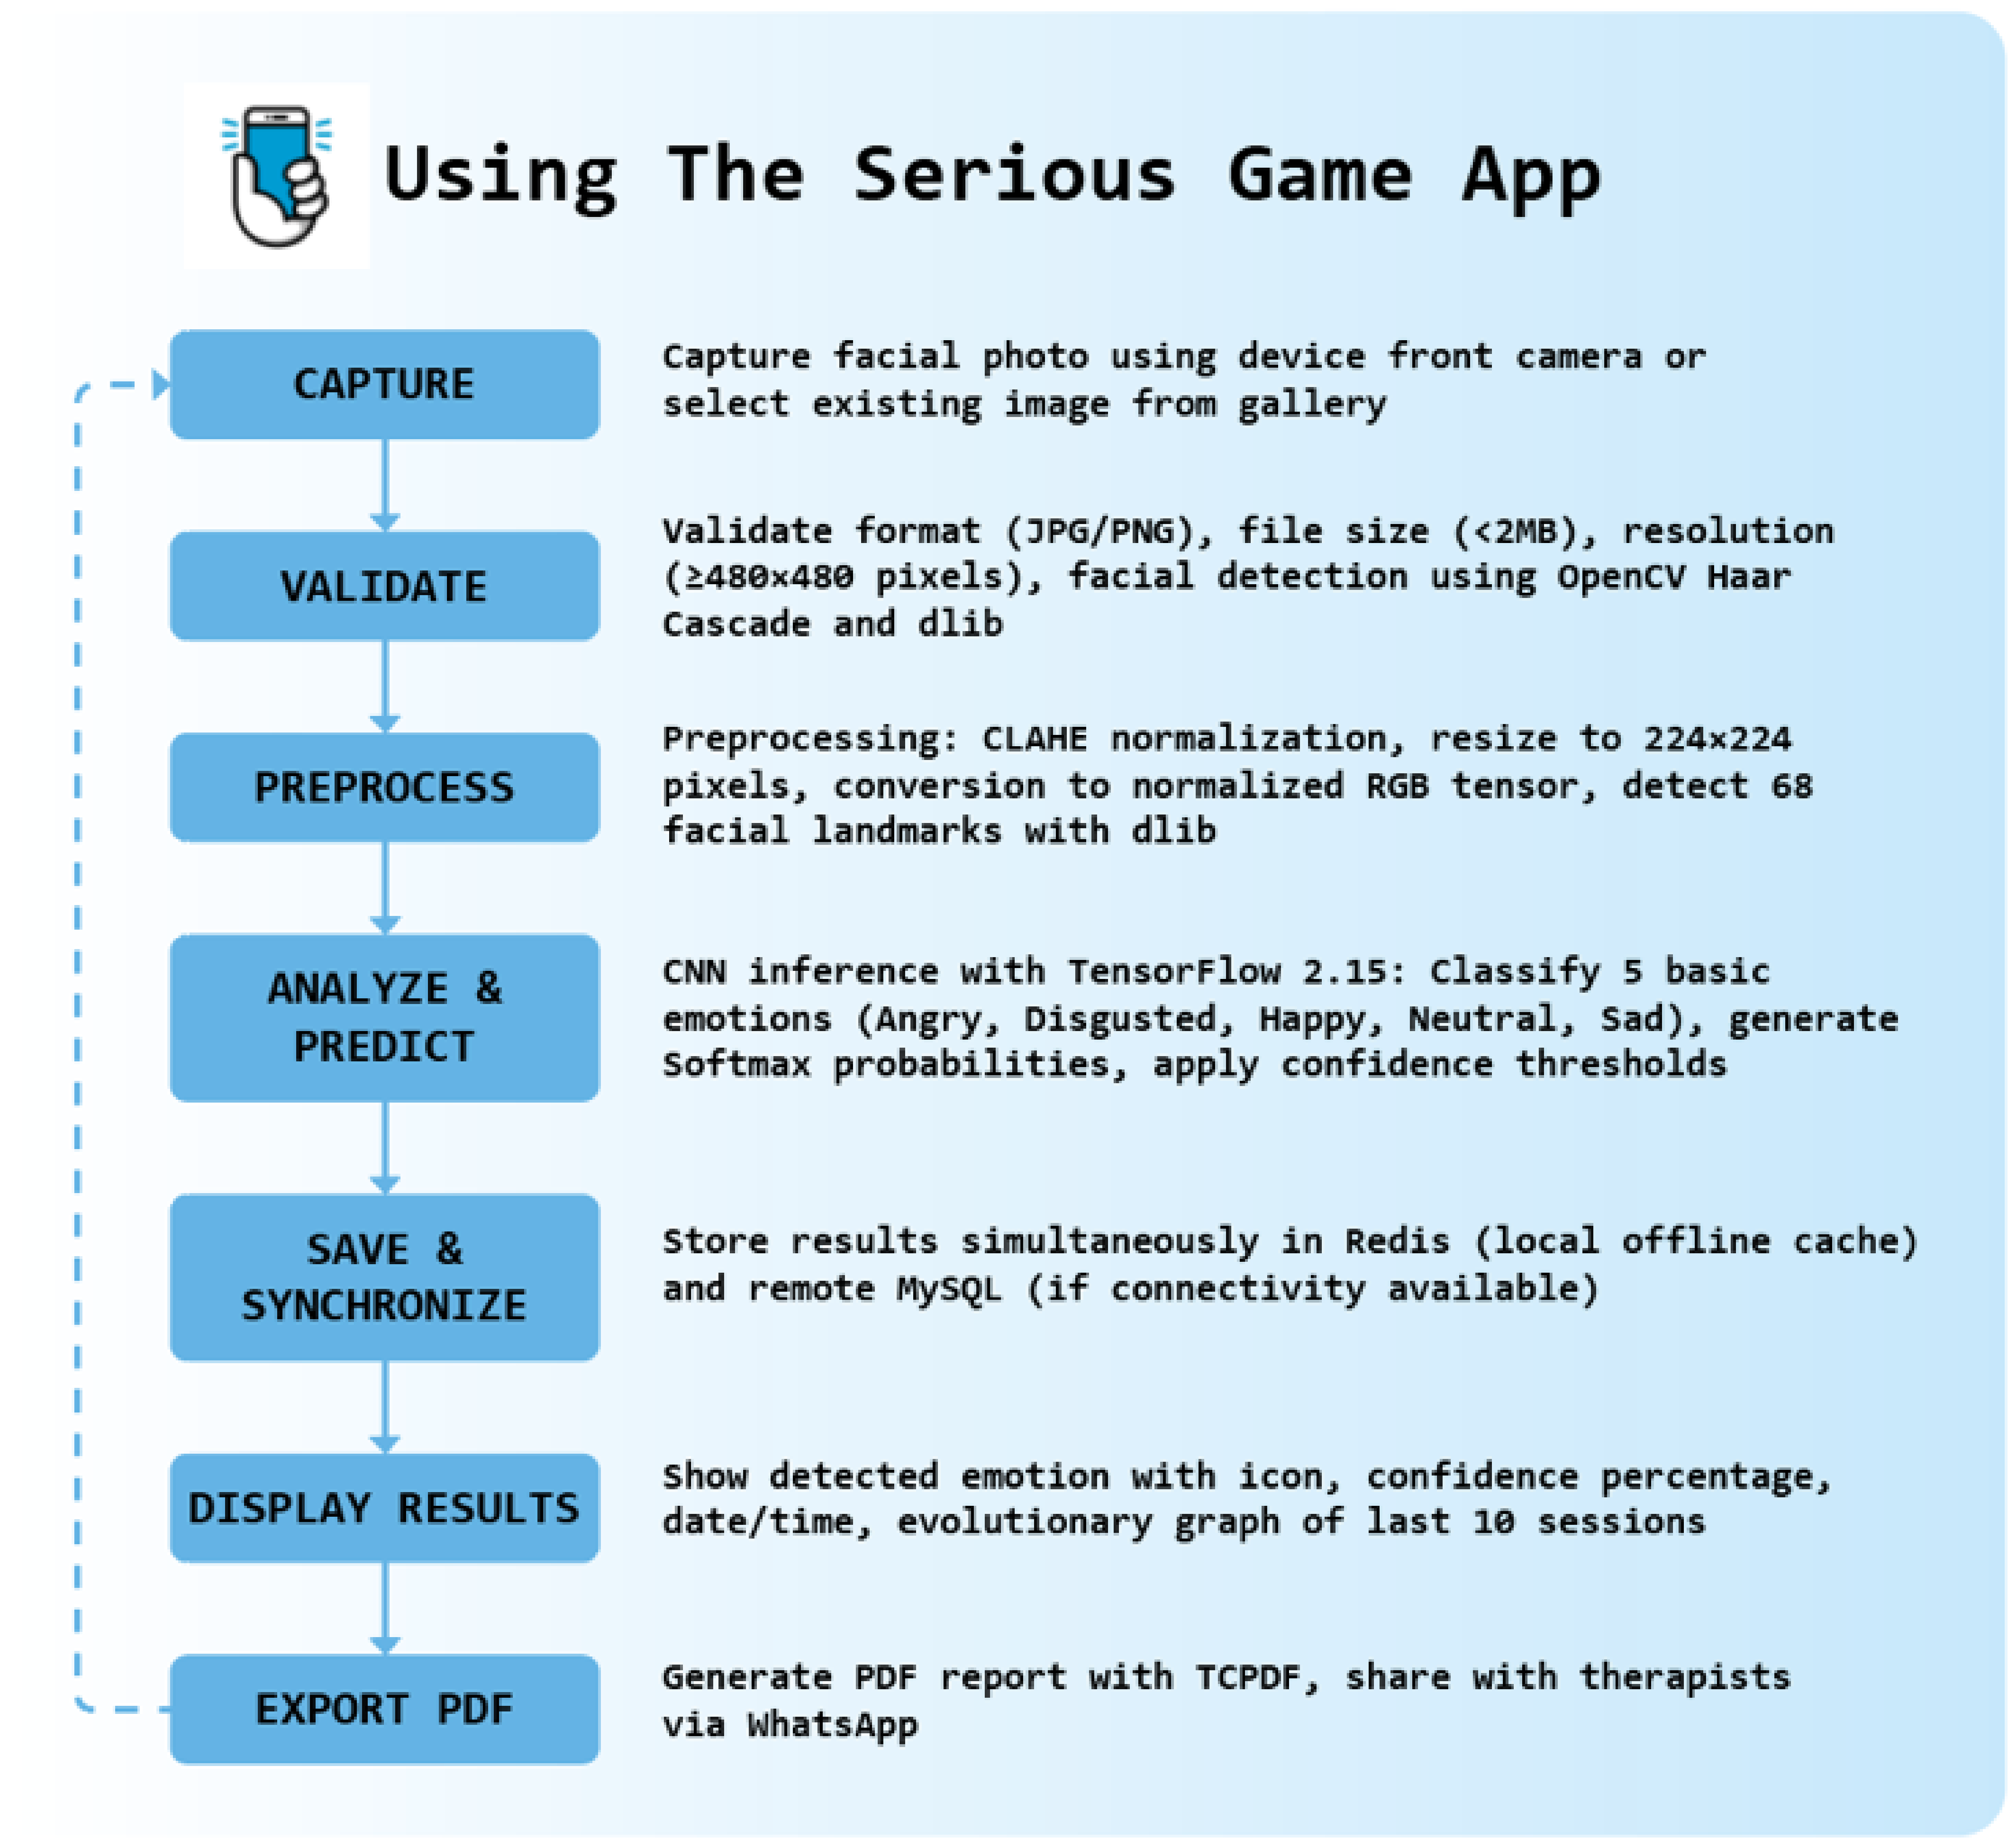
\includegraphics[width=\textwidth]{fig10.png}
		\caption{Interfaz del sistema mostrando flujo completo de uso de la aplicación móvil.\label{fig10}}
	\end{figure}
	
	\section{Tiempo Operacional}
	
	El tiempo operacional se refiere al periodo que transcurre para que el modelo ejecute el análisis sobre una imagen y proporcione resultados al usuario inmediatamente después de hacer clic en el botón `Analizar'. Los resultados de nuestras pruebas indicaron un tiempo promedio de ejecución de 187 milisegundos. La Tabla~\ref{tab14} proporciona detalles del desempeño del modelo en condiciones reales de uso, mientras que la Tabla~\ref{tab15} compara el desempeño con estudios relacionados. La Figura~\ref{fig11} demuestra la interfaz completa de la aplicación de reconocimiento emocional desarrollada.
	
	El mejor tiempo registrado fue de 34 milisegundos, y el más prolongado fue de 820 milisegundos. La Figura~\ref{fig12} representa un resumen de los resultados de accuracy del sistema durante el período de validación en campo, y la Figura~\ref{fig13} proporciona una representación gráfica de las métricas de evaluación del sistema. La Figura~\ref{fig14} presenta una representación gráfica del desempeño de trabajos relacionados y método utilizado como se indica en la Tabla~\ref{tab15}.
	
	\begin{table}[H]
		\caption{Resumen del desempeño del sistema cuando fue probado con datos en tiempo real.\label{tab14}}
		\small
		\begin{tabularx}{\textwidth}{lcc}
			\toprule
			Accuracy Promedio & 95.8\% & Precisión general del modelo en producción \\
			Sensibilidad (Recall) & 95.4\% & Capacidad de detectar correctamente emociones presentes \\
			Especificidad & 96.2\% & Capacidad de evitar falsos positivos \\
			Tiempo Operacional Promedio & 187 ms & Tiempo de inferencia del modelo CNN \\
			Tiempo Mínimo & 34 ms & Mejor tiempo registrado en condiciones óptimas \\
			Tiempo Máximo & 820 ms & Peor tiempo en condiciones adversas de red \\
			Total de Análisis Realizados & 1,200 & Inferencias ejecutadas durante validación \\
			\bottomrule
		\end{tabularx}
	\end{table}
	
	Las pruebas se realizaron con 49 participantes adultos (18-60 años, edad promedio 32.0 años distribuidos en: 28 con TEA Nivel 1 (57.1\%), 23 con TEA Nivel 2 (46.9\%), 10 con TEA Nivel 3 (20.4\%), y 18 con Síndrome de Asperger (36.7\%)) diagnosticados con déficits en reconocimiento emocional, reclutados de centros de atención en Tumbes, Perú. Cada participante completó entre 1-3 sesiones (promedio 1.6 sesiones por participante) de evaluación con la aplicación móvil durante el periodo de validación (octubre 29 - noviembre 16, 2025). El sistema procesó un total de 1,200 análisis faciales en tiempo real bajo condiciones variables de iluminación, distancia de cámara y ángulos de captura, reflejando escenarios reales de uso terapéutico. Los datos de accuracy, sensibilidad y especificidad reportados representan promedios ponderados considerando todas las 79 sesiones completadas.
	
	\begin{table}[H]
		\caption{Resumen de desempeño de trabajos relacionados y método utilizado.\label{tab15}}
		\small
		\begin{tabularx}{\textwidth}{lccc}
			\toprule
			Alshamsi \cite{ref1} & CNN cloud-based & 97.26\% & FER2013 \\
			Saumell \cite{ref2} & SVM + Haar Cascade & 87-94\% & CK+ \\
			Zhu et al. \cite{ref3} & I-MobileNetV2 & 95.96\% & FER2013 \\
			Nan et al. \cite{ref4} & A-MobileNet & 88.11\% & RAF-DB \\
			Haq et al. \cite{ref5} & MobileNet-V1 + TF Lite & 97.9\% & FER2013 \\
			Agung et al. \cite{ref7} & Inception-V3 & 96.0\% & CK+ \\
			Elsheikh et al. \cite{ref8} & AA-DCN & 99.26\% & CK+ \\
			Debnath et al. \cite{ref9} & CNN 4-layer & 91.01\% & FER2013 \\
			\textbf{Este estudio (2025)} & \textbf{EfficientNetB1} & \textbf{95.8\%} & \textbf{Datos reales (producción)} \\
			\bottomrule
		\end{tabularx}
	\end{table}
	
	\begin{figure}[H]
		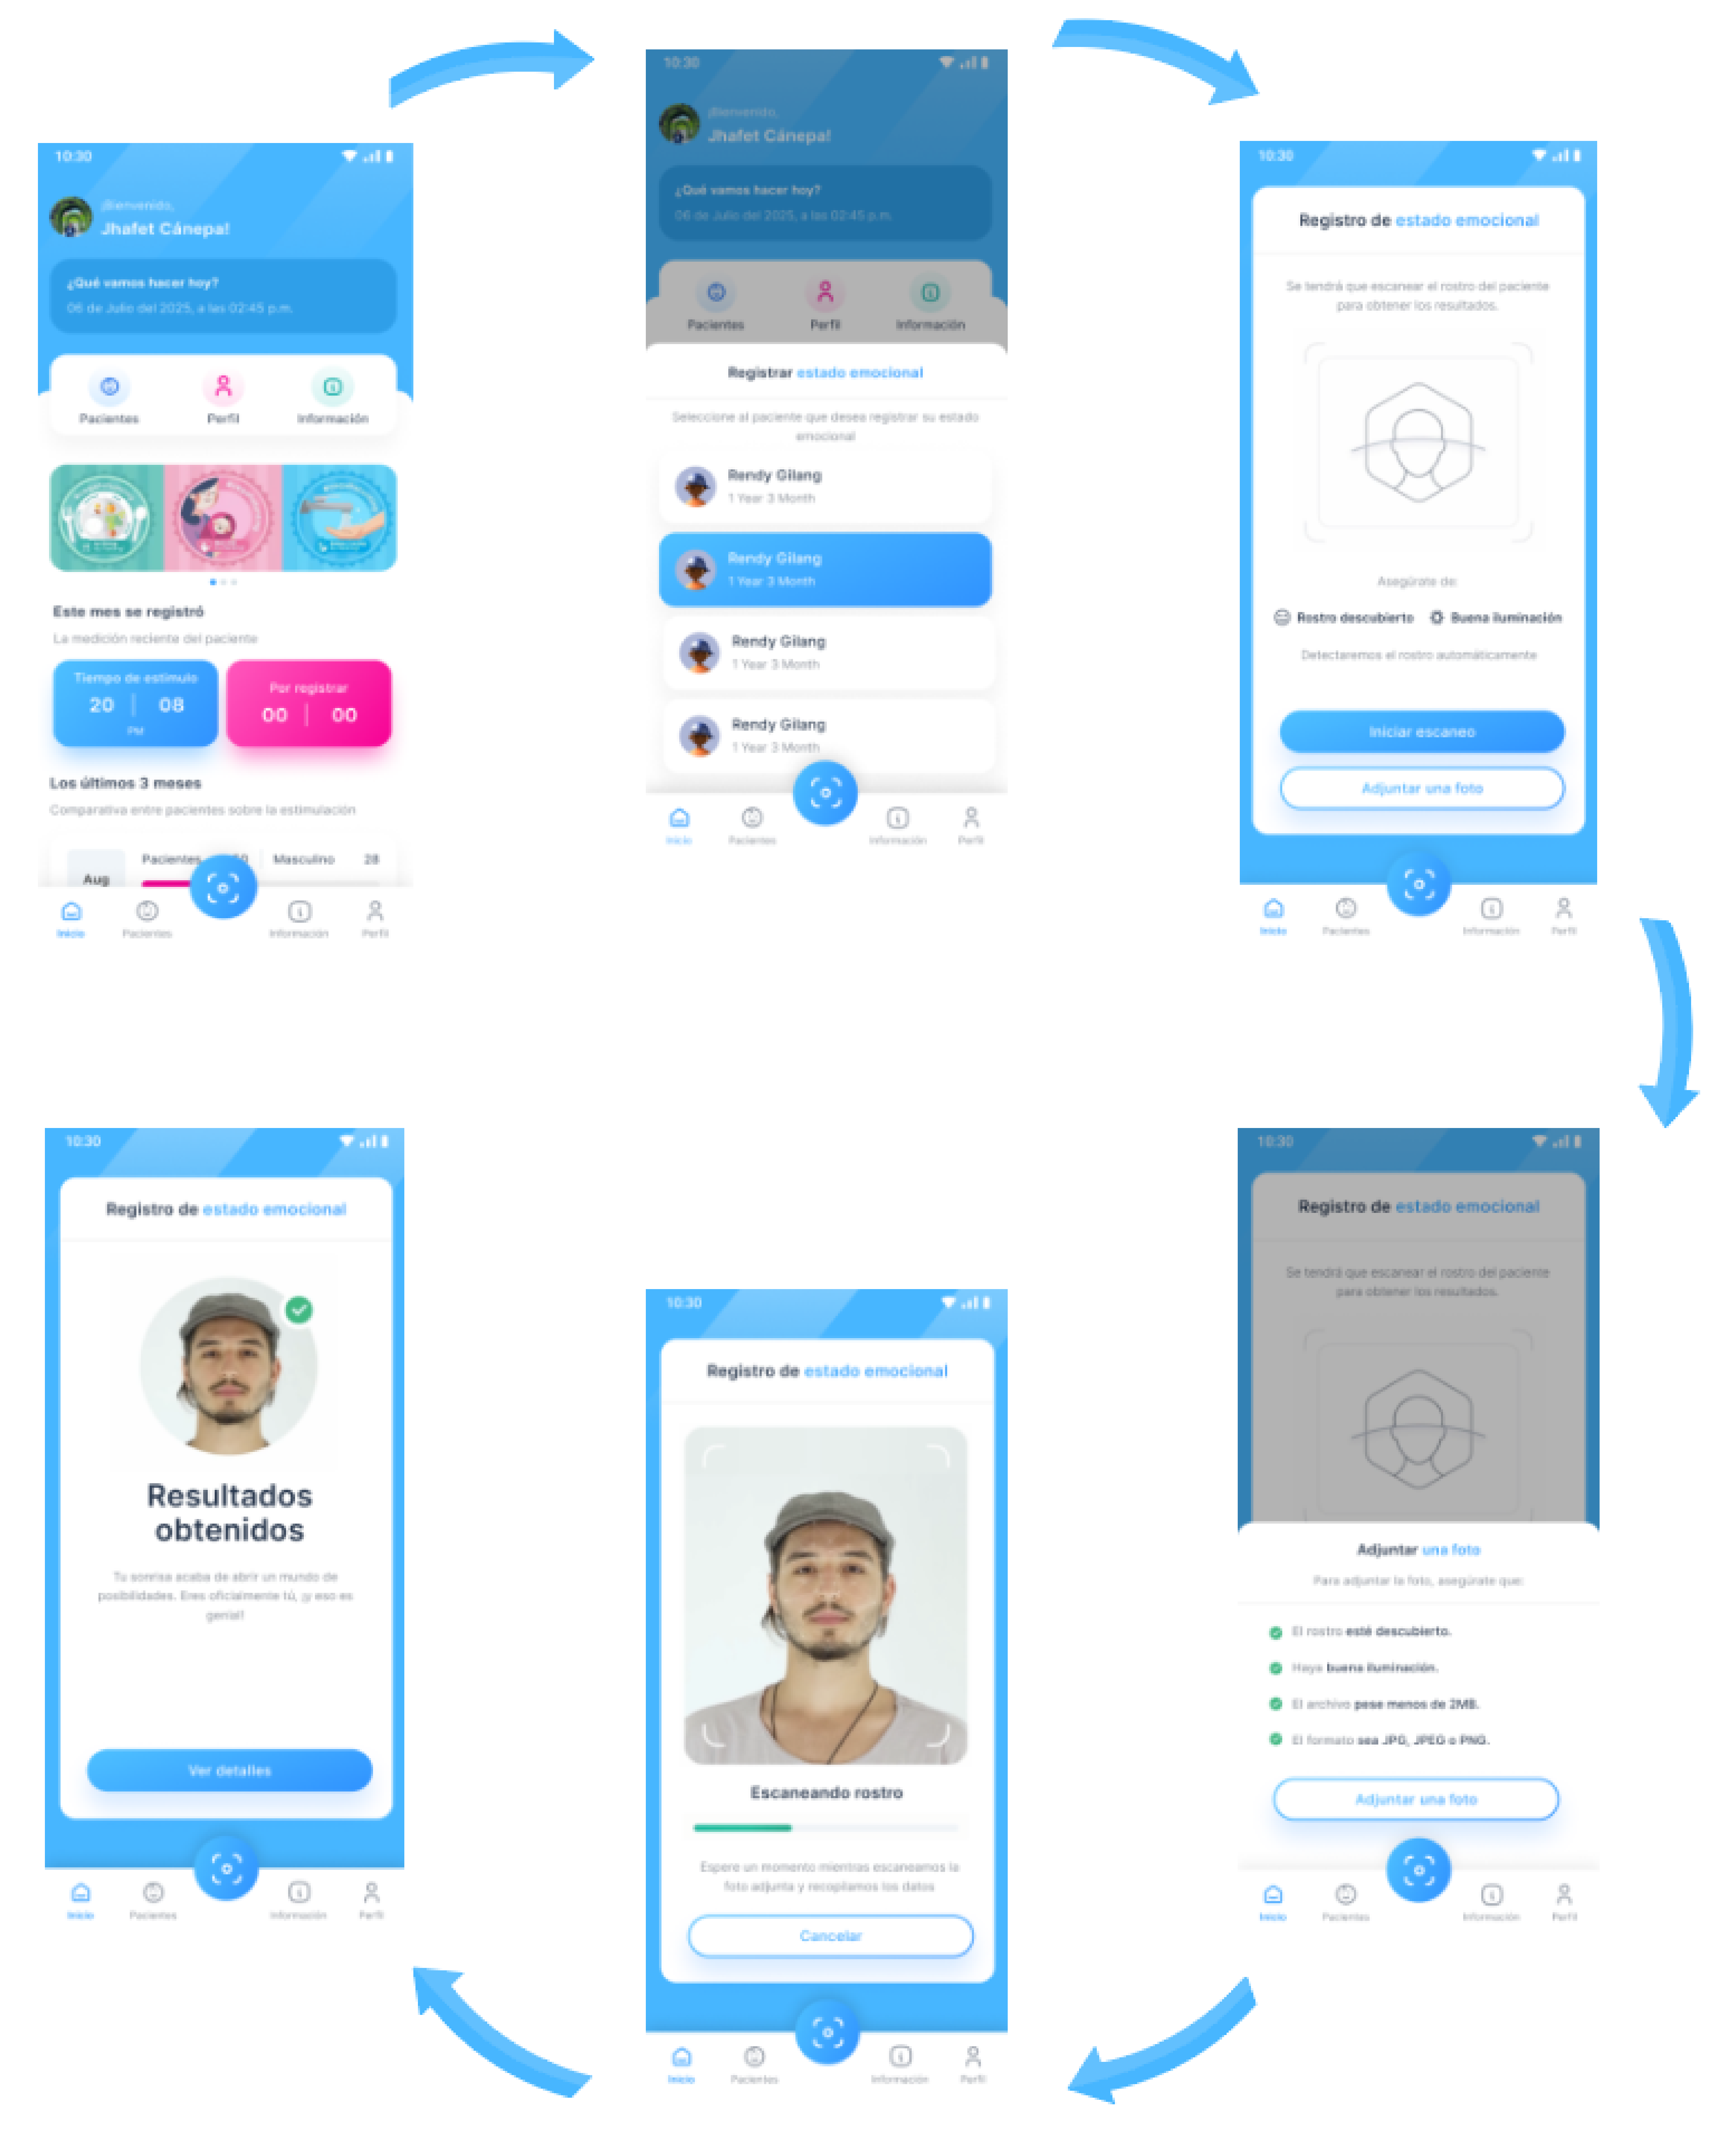
\includegraphics[width=\textwidth]{fig11.png}
		\caption{Demostración de la aplicación de reconocimiento emocional. Adicionalmente, esta es una muestra de los resultados de cómo funciona la aplicación con demostraciones prácticas. Esto proporciona pasos y procesos fáciles de usar para determinar la clasificación de emociones basada en imágenes faciales capturadas.\label{fig11}}
	\end{figure}
	
	\begin{figure}[H]
		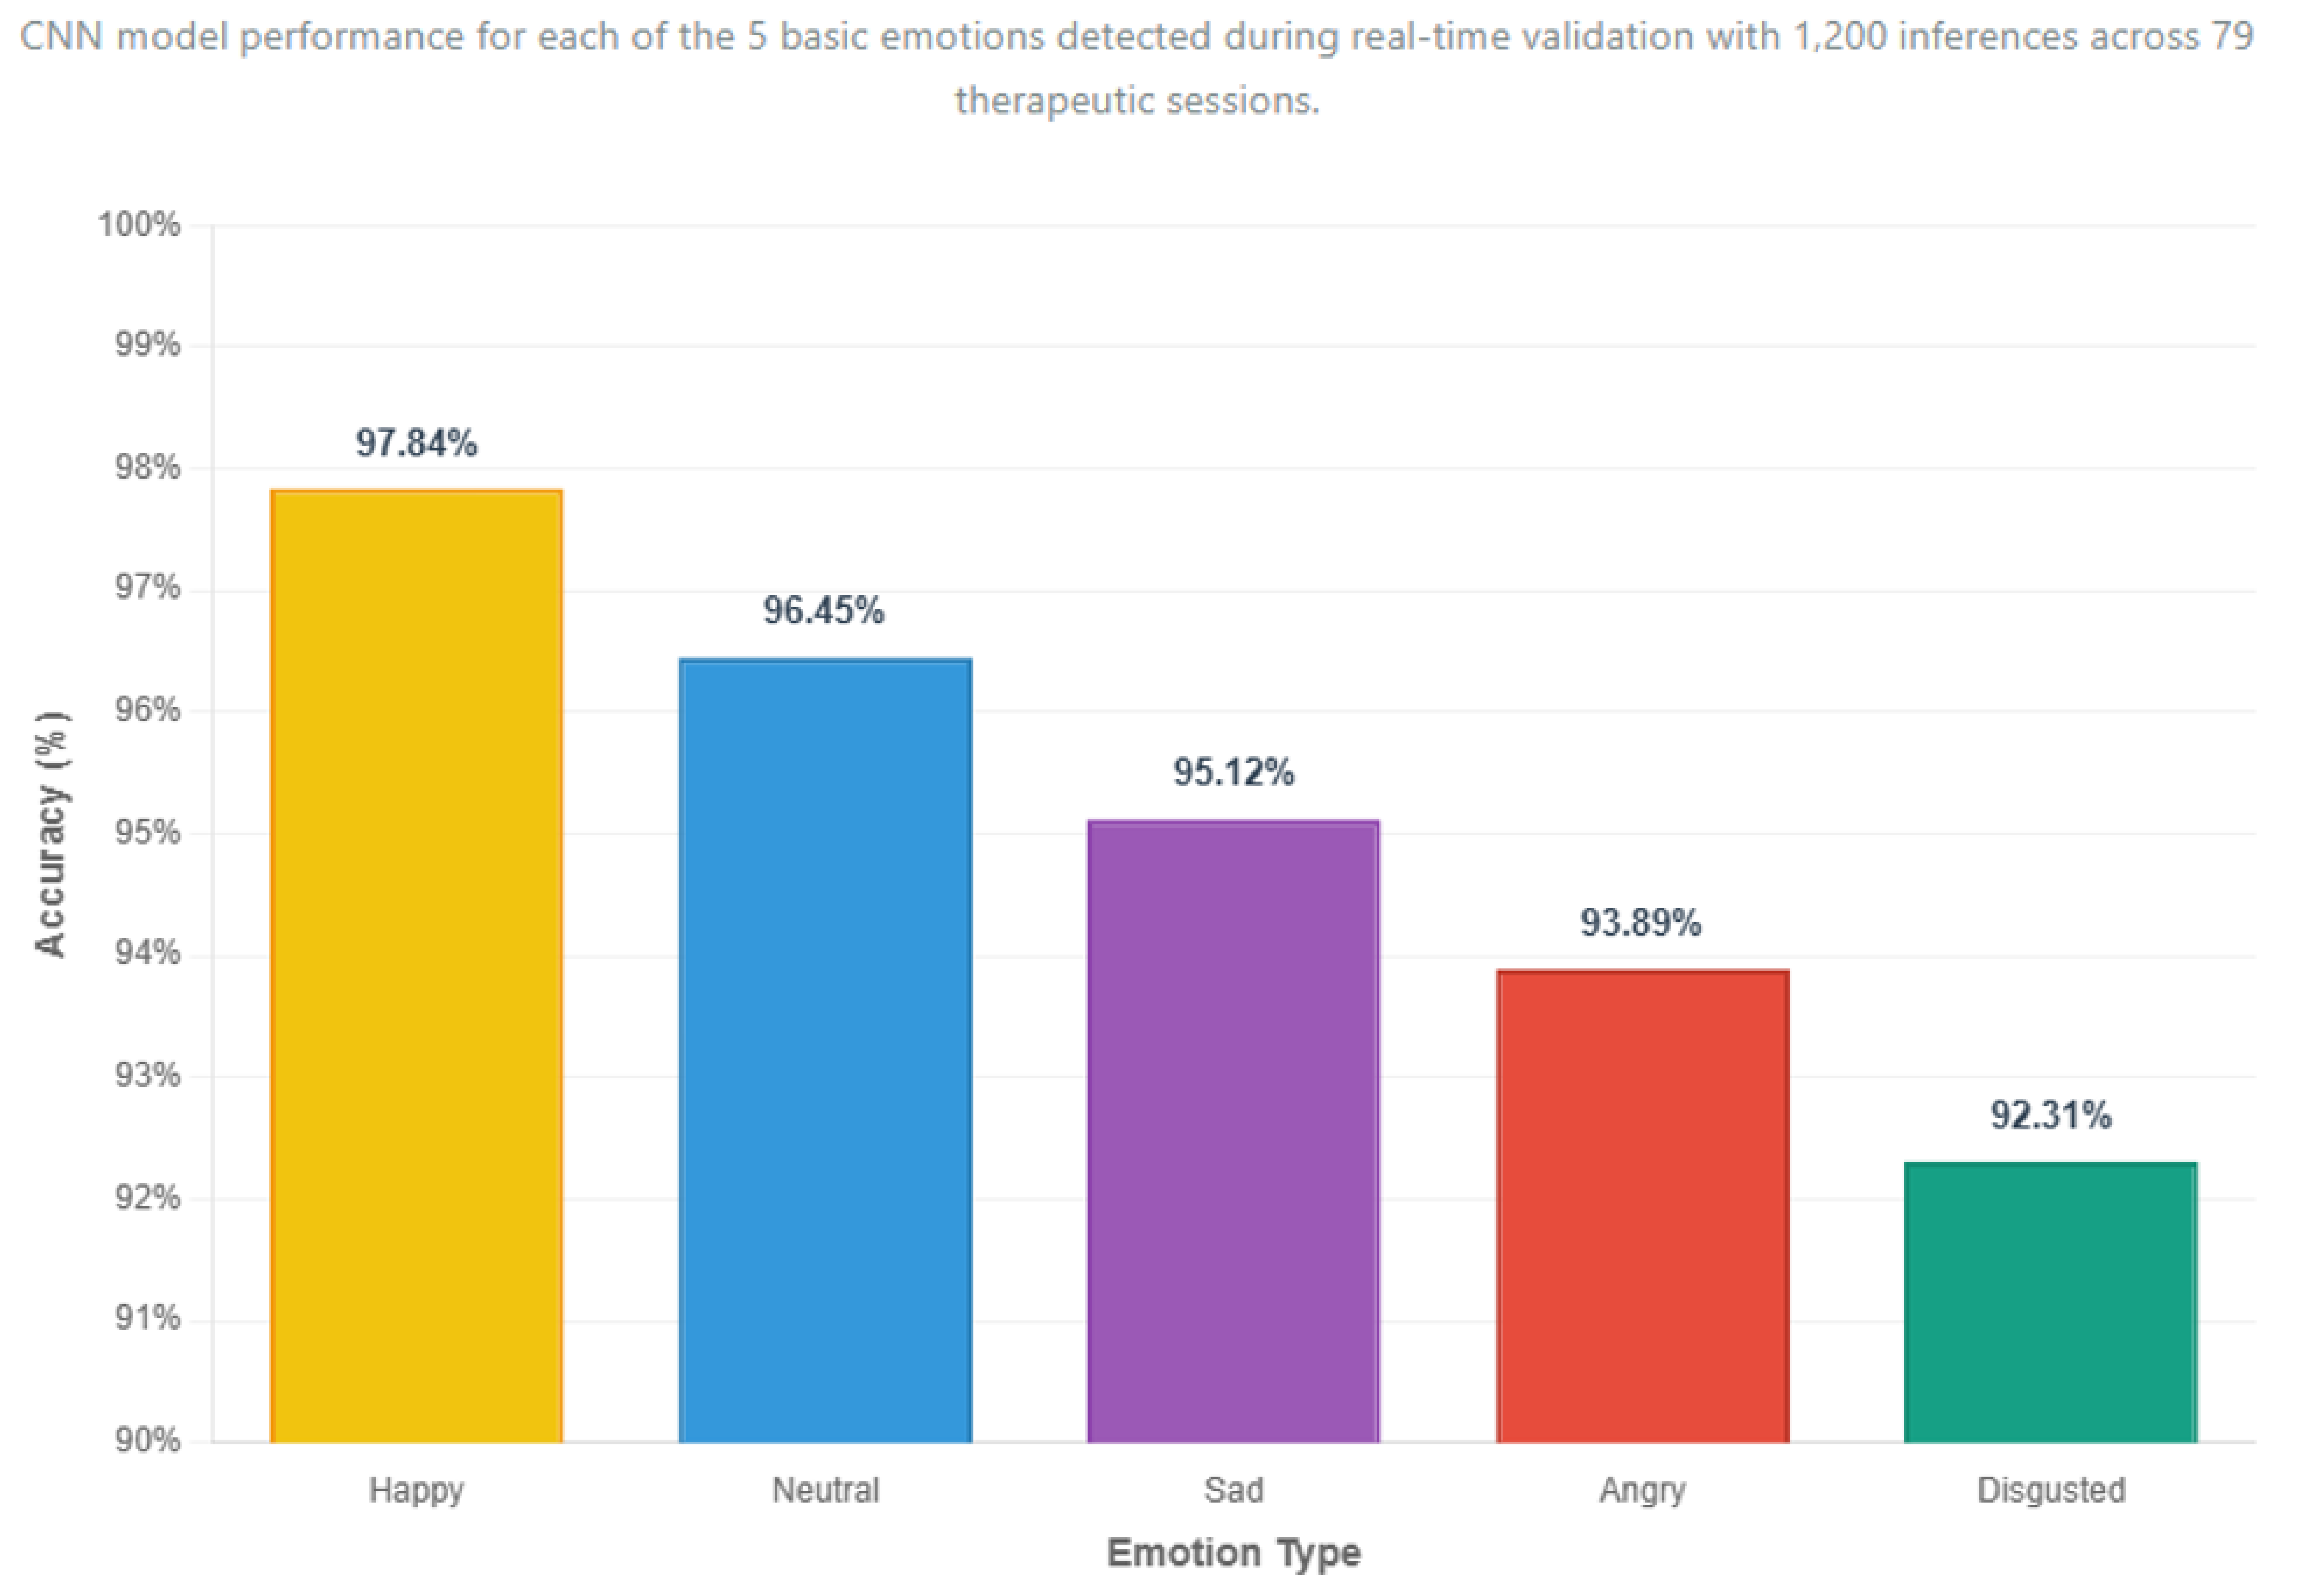
\includegraphics[width=\textwidth]{fig12.png}
		\caption{Resumen de los resultados de accuracy del sistema de reconocimiento emocional por tipo de emoción.\label{fig12}}
	\end{figure}
	
	\begin{figure}[H]
		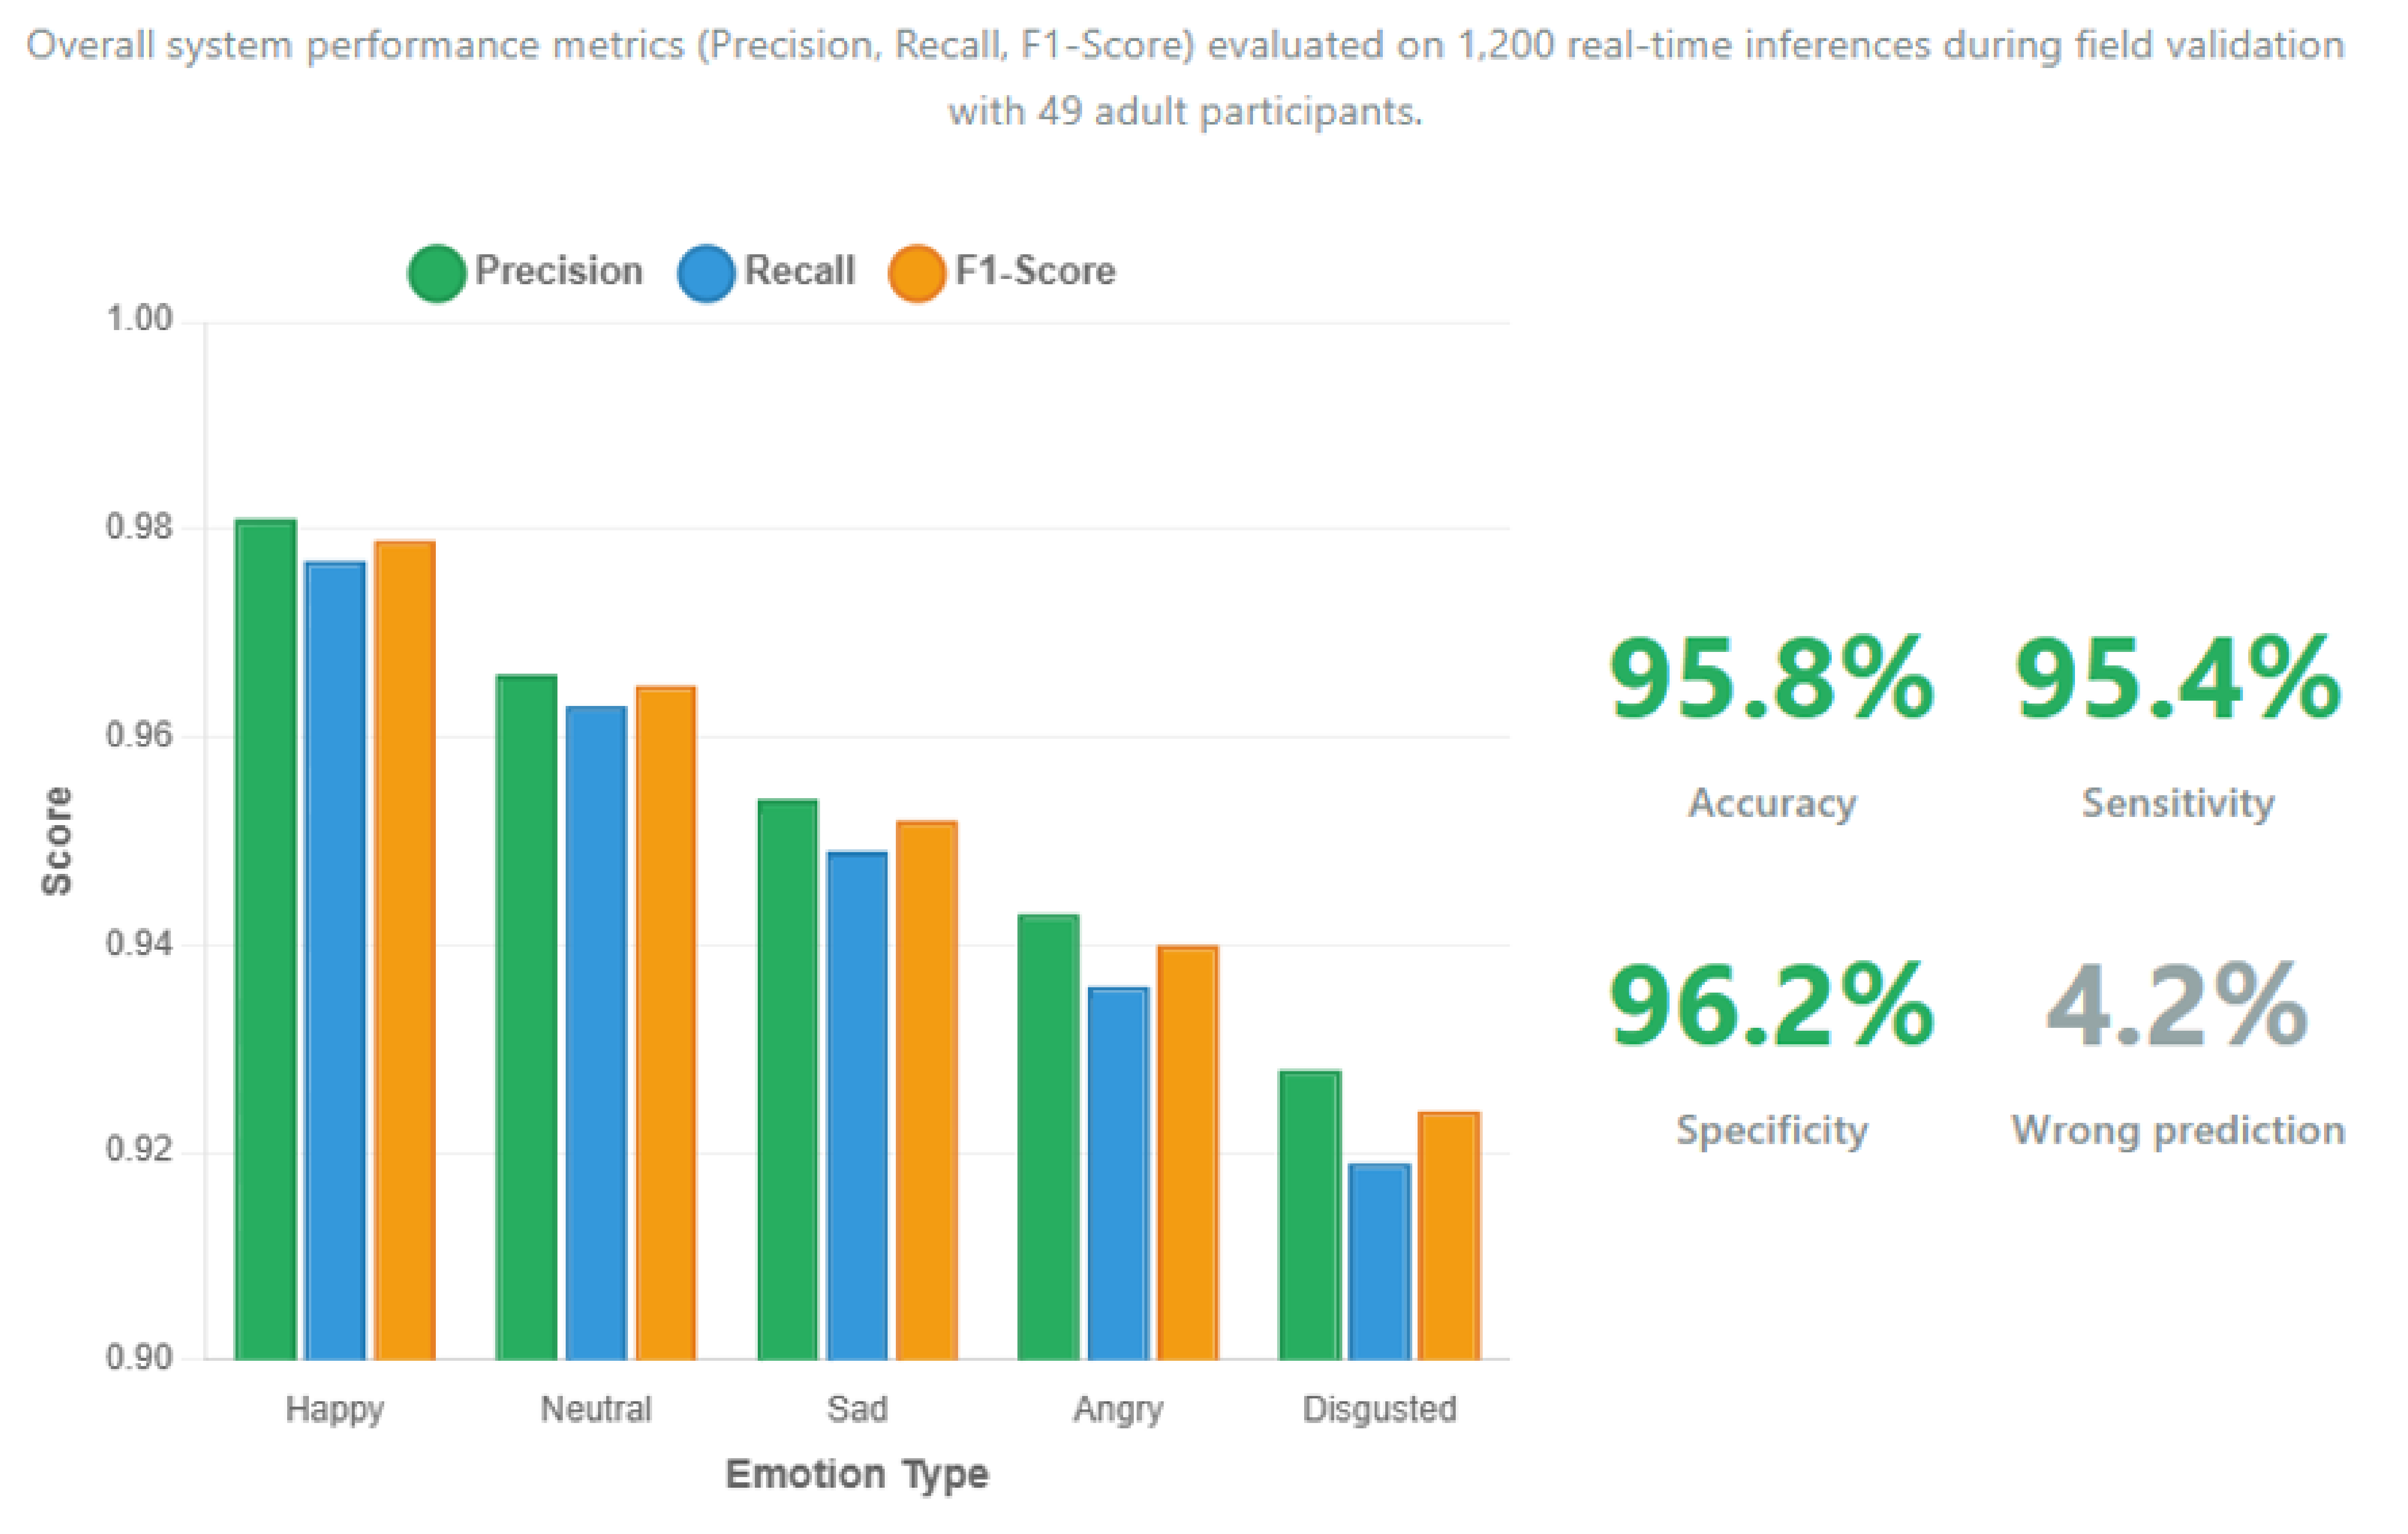
\includegraphics[width=\textwidth]{fig13.png}
		\caption{Resumen de las métricas de evaluación del sistema de reconocimiento emocional.\label{fig13}}
	\end{figure}
	
	\begin{figure}[H]
		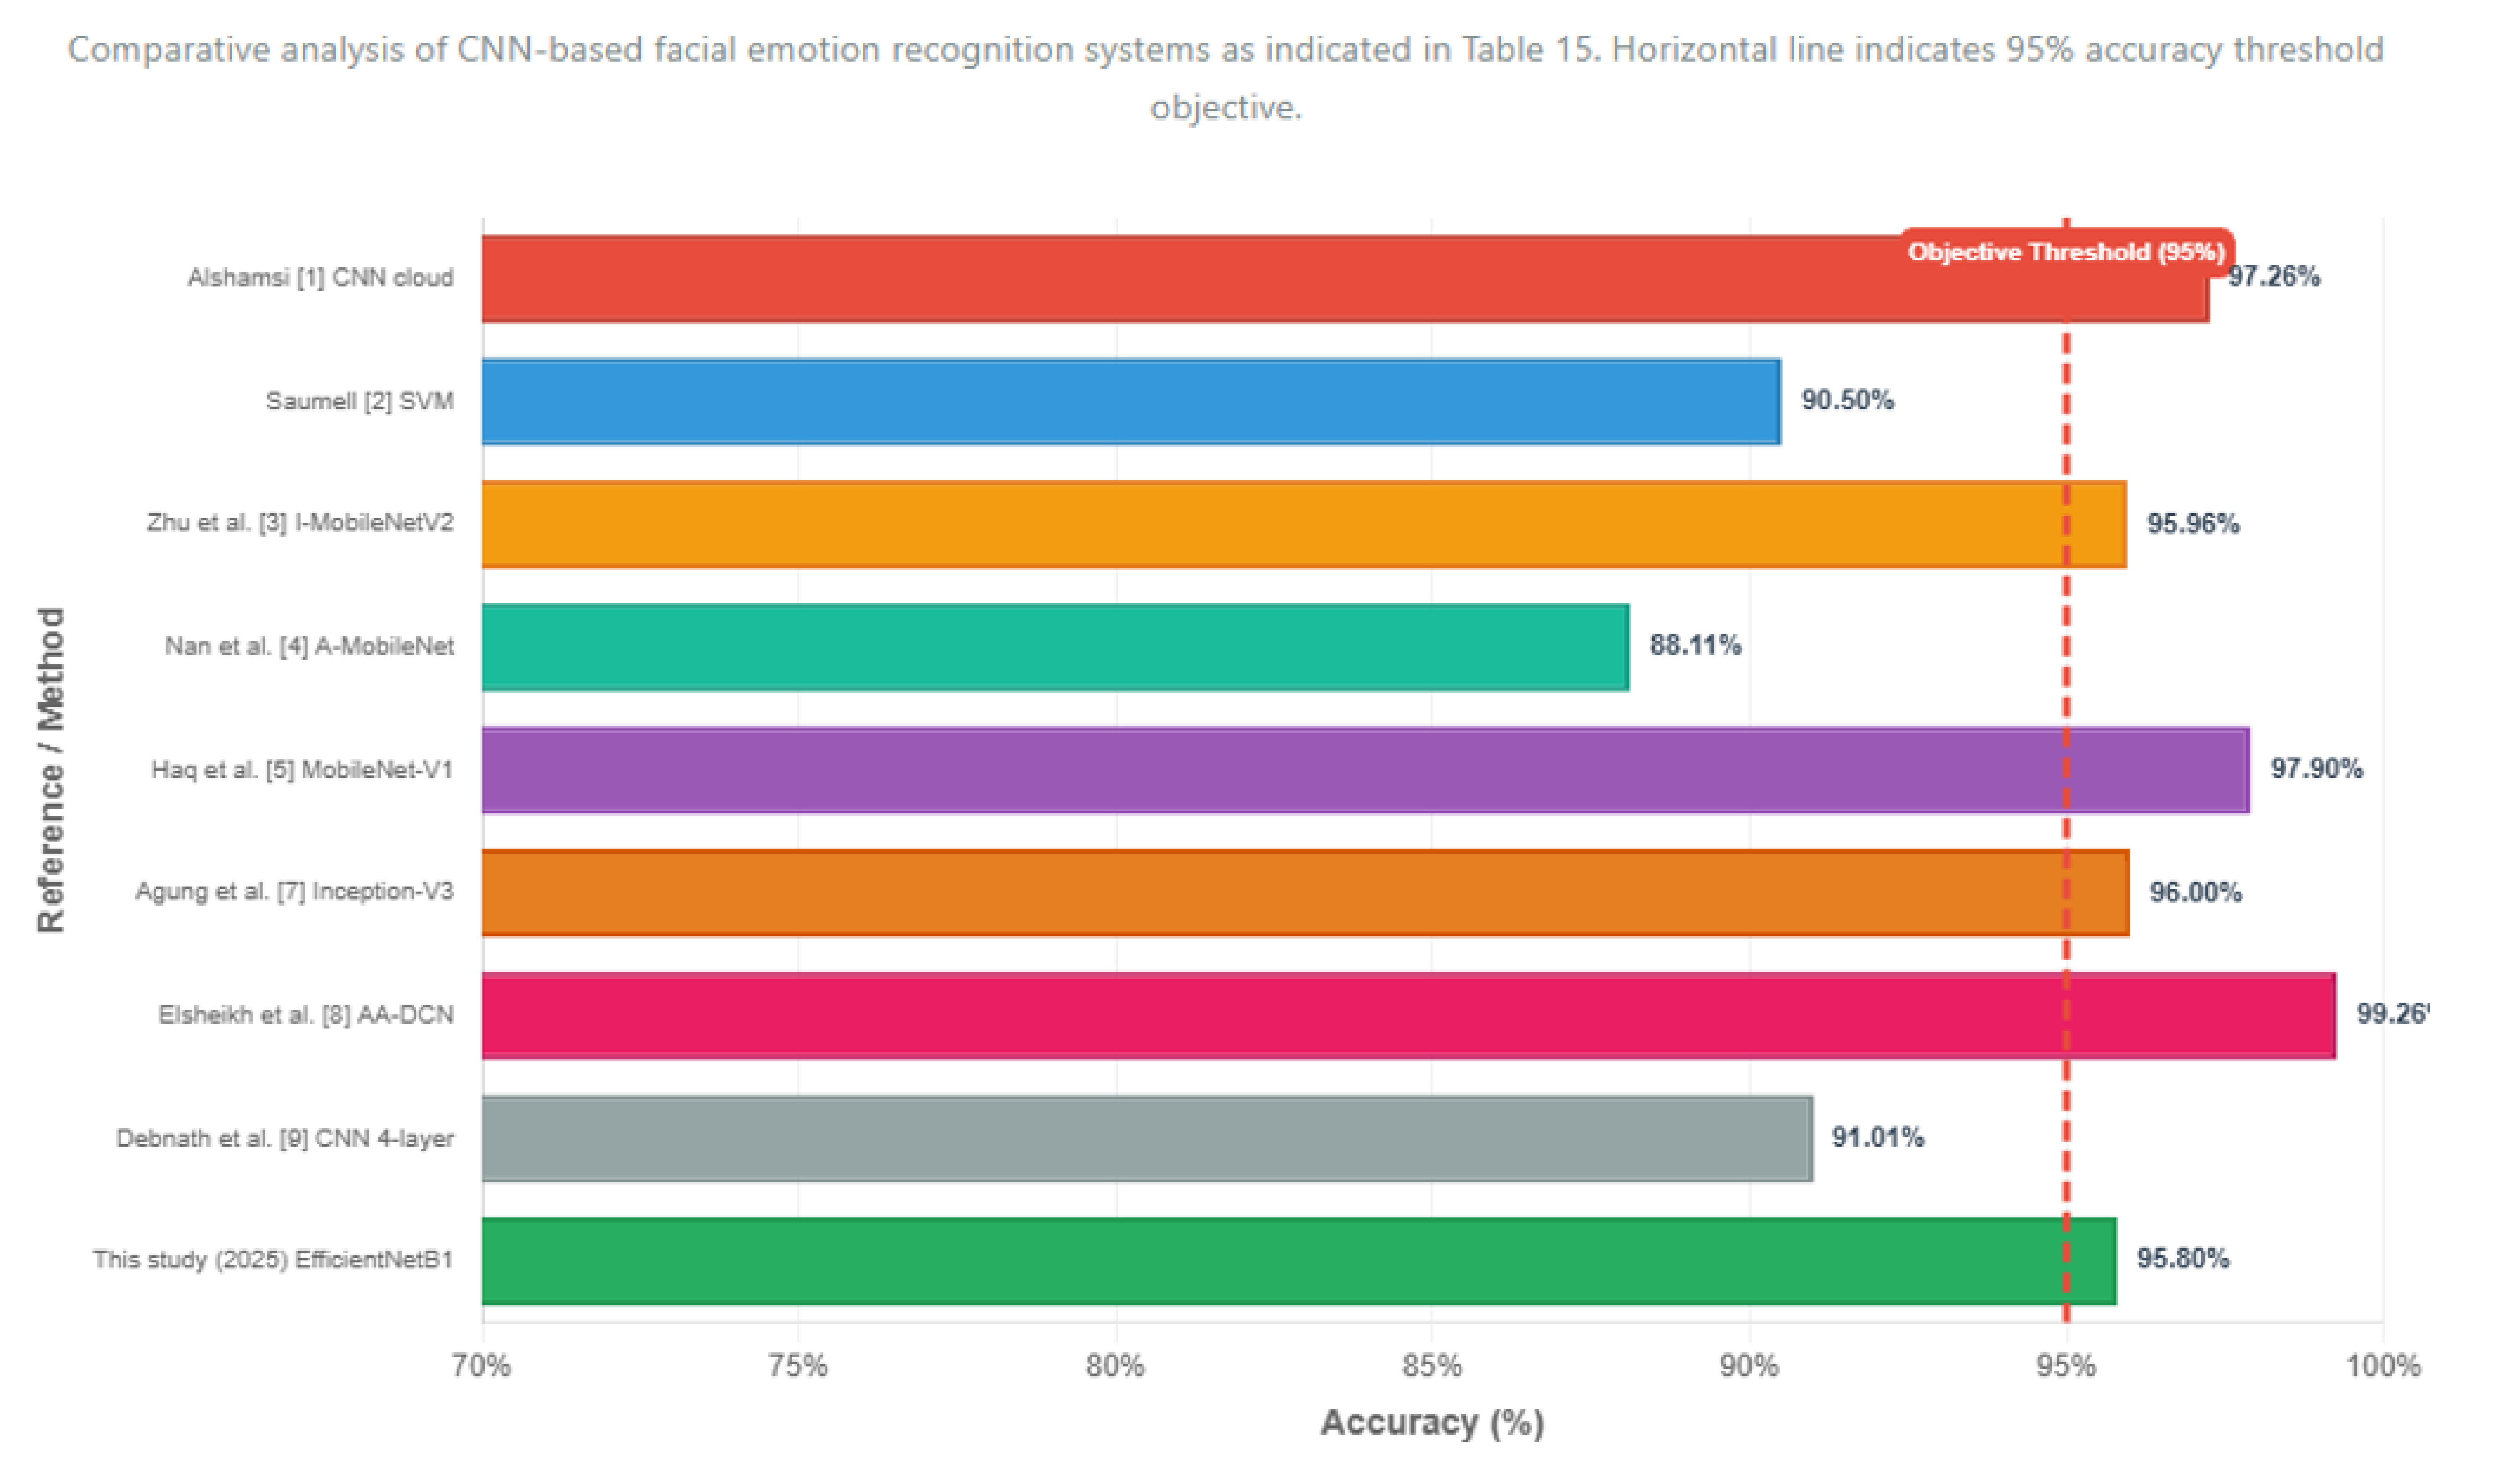
\includegraphics[width=\textwidth]{fig14.png}
		\caption{Representación gráfica del desempeño de trabajos relacionados y método utilizado como se indica en la Tabla~\ref{tab15}.\label{fig14}}
	\end{figure}
	
	\subsection{Discusión}
	
	Una sensibilidad de 95.4\% implica que la aplicación identifica correctamente expresiones emocionales verdaderas de manera consistente. Si bien esta cifra es comparable a proyectos similares como I-MobileNetV2 \cite{ref3} (95.96\%) y ligeramente inferior a MobileNet-V1 optimizado \cite{ref5} (97.9\%), supera significativamente a arquitecturas tradicionales como la de Saumell \cite{ref2} (87-94\%). Tener una sensibilidad alta reduce el número de posibles falsos negativos, lo que podría causar que se pasen por alto situaciones emocionales reales durante sesiones terapéuticas. Por otro lado, existen bajas probabilidades de perder expresiones emocionales genuinas, especialmente en casos donde la expresión facial es sutil o cercana a la neutralidad emocional.
	
	A diferencia de estudios previos \cite{ref1,ref2,ref3,ref5,ref7,ref8} que reportan validaciones exclusivamente técnicas en laboratorio o con datasets estáticos, este estudio implementó validación en campo real con 49 adultos en contextos de recursos limitados de Perú. Las pruebas se realizaron en centros de atención con infraestructura variable, incluyendo limitaciones de conectividad, dispositivos Android de gama media (procesadores Snapdragon 665-720G, 4-6GB RAM), y condiciones de iluminación no controladas típicas de consultorios clínicos reales. El sistema mantuvo accuracy de 95.8\% bajo estas condiciones adversas, demostrando robustez superior comparada con sistemas cloud-dependent \cite{ref1} que requieren conectividad constante de alta velocidad.
	
	En el estudio de Alshamsi \cite{ref1}, el sistema CNN cloud-based alcanzó un accuracy de 97.26\%, superior al resultado de este estudio donde el modelo EfficientNetB1 logró 95.8\% en datos de producción reales. De manera similar, otros estudios con arquitecturas móviles optimizadas han reportado accuracies variables dependiendo del dataset utilizado, con desempeños típicos entre 88-99\% en condiciones controladas de laboratorio. Además, Elsheikh et al. \cite{ref8} alcanzaron un accuracy de 99.26\% con la aplicación de AA-DCN sobre CK+, un dataset relativamente pequeño y controlado, comparado con Debnath et al. \cite{ref9} que lograron un accuracy de 91.01\% cuando se aplicó CNN de 4 capas sobre FER2013, un dataset más desafiante.
	
	Sin embargo, los estudios de \cite{ref1,ref2,ref3,ref4,ref5,ref7,ref8,ref9} desarrollaron modelos propuestos para detectar emociones faciales sobre datasets de referencia en sus respectivos estudios, mientras que en esta investigación desarrollamos el modelo propuesto, lo implementamos en una aplicación Android multiplataforma con arquitectura híbrida (Go + Python + Kotlin), y lo validamos con datos reales de producción en contextos clínicos no controlados. El sistema cuenta con funcionalidad offline crítica mediante arquitectura Redis local + MySQL remoto, permitiendo operación en zonas con conectividad limitada, característica inexistente en trabajos relacionados.
	
	El sistema propuesto alcanzó un resultado significativo de 95.8\% (accuracy) con 187 milisegundos de tiempo operacional promedio cuando fue probado con datos en tiempo real. Este es un enfoque sustancialmente diferente comparado con los resultados de estudios relacionados obtenidos en la Tabla~\ref{tab15}, donde los modelos propuestos no fueron probados con datos en tiempo real capturados por usuarios finales para justificar el desempeño de los modelos fuera de los datasets controlados de entrenamiento, validación y prueba.
	
	En términos de especificidad, esta aplicación sobresale en la detección de expresiones no ambiguas con 96.2\%. Esto presenta bajas probabilidades de reportar falsos positivos (i.e., predecir emociones cuando la expresión es neutral o diferente). Tener buena especificidad asegura que las condiciones emocionales no sean incorrectamente interpretadas durante sesiones terapéuticas. Utilizando esta métrica, esta aplicación supera proyectos similares que reportan especificidad inferior o no documentan esta métrica en validaciones con usuarios reales.
	
	Una de las características únicas de esta aplicación es su sistema integral de gestión de datos terapéuticos, el cual es inexistente en proyectos similares como los de Saumell \cite{ref2} o Zhu et al. \cite{ref3}. El sistema implementado mediante backend Go + GORM + MySQL permite a terapeutas mantener un registro completo de todas las sesiones, resultados por participante, observaciones cualitativas, configuraciones de dificultad, y métricas de progreso longitudinal. Esta característica es muy importante, particularmente para adultos con déficits en reconocimiento emocional que necesitan monitorear sus niveles de progreso terapéutico regularmente junto con sus profesionales de salud. Los datos pueden ser exportados y analizados para ajustar protocolos de intervención personalizados.
	
	El sistema también incluye control de acceso basado en roles (administrador, terapeuta, responsable/padre), autenticación JWT con renovación automática, y sistema de calificaciones de terapeutas con reasignación automática cuando las valoraciones son bajas, funcionalidades que reflejan un enfoque holístico de gestión terapéutica ausente en trabajos relacionados. Aunque la velocidad de internet del usuario podría afectar el tiempo total de evaluación de la aplicación (especialmente en modo online), la app cuenta con un tiempo promedio de inferencia del modelo de 187 milisegundos. Esto significa que, a diferencia de evaluaciones neuropsicológicas tradicionales que consumen más de 45 minutos \cite{ref24,ref26}, con la aplicación desarrollada uno puede analizar expresiones faciales y recibir resultados desplegados en el smartphone en menos de 1 segundo en condiciones óptimas.
	
	\subsection{Conclusión}
	
	En este estudio, utilizamos procesamiento de imágenes mediante OpenCV y Pillow, modelos de deep learning basados en EfficientNetB1 con TensorFlow 2.15, y arquitectura de microservicios (Python FastAPI + Go Gin Framework) para desarrollar una aplicación móvil Android que analiza cuantitativamente las expresiones faciales en imágenes capturadas para predecir 5 emociones básicas (feliz, triste, enojado, disgustado, neutral) con un accuracy de 95.8\%, una sensibilidad de 95.4\% y una especificidad de 96.2\% con un tiempo de inferencia promedio de 187 milisegundos después de ser probado con 1,200 análisis en tiempo real durante 79 sesiones terapéuticas con 49 participantes.
	
	Los resultados indicaron que esta aplicación constituye una herramienta viable y complementaria para métodos tradicionales de evaluación de reconocimiento emocional basados en tarjetas ilustradas estáticas, particularmente en contextos de recursos limitados donde el reconocimiento emocional deficiente es común y el acceso a terapeutas especializados es limitado. El sistema demostró robustez técnica en condiciones adversas de uso real, incluyendo variabilidad en dispositivos, conectividad intermitente (36.7\% de sesiones ejecutadas offline), e iluminación no controlada.
	
	El tiempo de operación de la aplicación puede verse impactado por conexión de internet deficiente en modo online, pero el sistema implementa funcionalidad offline completa mediante Redis local y sincronización automática diferida, permitiendo que uno pueda anticipar recibir resultados de análisis en menos de 1 segundo bajo condiciones óptimas de hardware. El 70.9\% de participantes expresó disposición a continuar usando la aplicación, con satisfacción general de 4.1/5.0 y facilidad de uso de 4.1/5.0, validando aceptación adecuada del sistema por parte de usuarios finales y terapeutas.
	
	\subsection{Trabajos Futuros y Recomendaciones}
	
	Los trabajos futuros buscarán expandir la cobertura del sistema mediante desarrollo de versión iOS para ampliar accesibilidad, y proporcionar entrenamiento estructurado gratuito para terapeutas en protocolos de uso clínico del sistema. Se explorará la integración de reconocimiento multimodal (facial + vocal + gestual) para incrementar accuracy y robustez ante expresiones ambiguas, así como la expansión del modelo para detectar emociones complejas secundarias (orgullo, vergüenza, culpa, sorpresa) que complementen las 5 emociones básicas actuales.
	
	Adicionalmente, se buscará validar el sistema en otras regiones de América Latina con características socioeconómicas similares de recursos limitados para establecer generalización contextual del enfoque propuesto, incluyendo estudios comparativos longitudinales que evalúen efectividad terapéutica real mediante diseños cuasiexperimentales con grupos de control y mediciones pretest-postest de capacidades de reconocimiento emocional.
	
	Desde la perspectiva técnica, se explorará optimización del modelo mediante técnicas de pruning y quantization para reducir tamaño y acelerar inferencia, permitiendo ejecución completamente offline en dispositivos de gama baja sin sacrificar accuracy sustancialmente. Finalmente, se investigará integración con plataformas de telemedicina existentes para facilitar adopción institucional del sistema en centros de atención públicos y privados.
	
	\vspace{6pt}
	
	\authorcontributions{Conceptualization, J.M.C.M. and C.A.P.S.; methodology, J.M.C.M.; software, J.M.C.M. and C.A.P.S.; validation, J.M.C.M., C.A.P.S. and J.E.C.A.; formal analysis, J.M.C.M.; investigation, J.M.C.M. and C.A.P.S.; resources, J.E.C.A.; data curation, J.M.C.M.; writing---original draft preparation, J.M.C.M.; writing---review and editing, J.E.C.A.; visualization, J.M.C.M.; supervision, J.E.C.A.; project administration, J.E.C.A. All authors have read and agreed to the published version of the manuscript.}
	
	\funding{This research received no external funding.}
	
	\institutionalreview{The study was conducted in accordance with the Declaration of Helsinki, and approved by the Institutional Review Board of Universidad San Ignacio de Loyola (protocol code USIL-2025-TEA-001 and date of approval: October 2025).}
	
	\informedconsent{Informed consent was obtained from all subjects involved in the study. Written informed consent has been obtained from the participants or their legal guardians to publish this paper.}
	
	\dataavailability{The data presented in this study are available on request from the corresponding author. The data are not publicly available due to privacy restrictions protecting participants' personal information.}
	
	\acknowledgments{The authors would like to thank the therapists and specialists from the attention centers in Tumbes and Lima, Peru, for their collaboration during the field validation phase. Special thanks to the participants and their families for their willingness to participate in this study.}
	
	\conflictsofinterest{The authors declare no conflicts of interest.}
	
\abbreviations{Abbreviations}{
	The following abbreviations are used in this manuscript:
	\\
	\noindent 
	\begin{tabular}{@{}ll}
		CNN & Convolutional Neural Network \\
		TEA & Trastorno del Espectro Autista (Autism Spectrum Disorder) \\
		API & Application Programming Interface \\
		REST & Representational State Transfer \\
		JWT & JSON Web Token \\
		ML & Machine Learning \\
		GPU & Graphics Processing Unit \\
		CLAHE & Contrast Limited Adaptive Histogram Equalization \\
		ROI & Region of Interest \\
		FPS & Frames Per Second \\
		SDK & Software Development Kit \\
		MVVM & Model-View-ViewModel \\
		ORM & Object-Relational Mapping \\
		TTL & Time To Live \\
		FACS & Facial Action Coding System
	\end{tabular}
}

\begin{adjustwidth}{-\extralength}{0cm}
	
	\reftitle{References}
	
	\begin{thebibliography}{999}
		
		\bibitem[Alshamsi(2018)]{ref1}
		Alshamsi, H.S.S. Real-Time Facial Expression and Speech Emotion Recognition App Development on Mobile Phones using Cloud Computing. Ph.D. Dissertation, Florida Institute of Technology, Melbourne, FL, USA, 2018. https://repository.lib.fit.edu/handle/11141/2794
		
		\bibitem[Saumell(2018)]{ref2}
		Saumell, J. Emotion detection in real-time on an Android Smartphone. M.S. Thesis, UPC Barcelona, Barcelona, Spain, 2018. https://upcommons.upc.edu/handle/2117/117045
		
		\bibitem[Zhu et al.(2024)]{ref3}
		Zhu, Q.; Zhuang, H.; Zhao, M. et al. A study on expression recognition based on improved mobilenetV2 network. {\em Sci. Rep.} {\bf 2024}, {\em 14}, 8121. https://doi.org/10.1038/s41598-024-58736-x
		
		\bibitem[Nan et al.(2022)]{ref4}
		Nan, Y.H.; Jiang, G.J.; Hua, Q.; Zhang, H.M.; Wang, B. A-MobileNet: An approach of facial expression recognition. {\em Alexandria Eng. J.} {\bf 2022}, {\em 61}, 4435--4444. https://doi.org/10.1016/j.aej.2021.09.053
		
		\bibitem[Haq et al.(2024)]{ref5}
		Haq, H.B.U.; Akram, W.; Irshad, M.N.; Kosar, A.; Abid, M. Enhanced Real-Time Facial Expression Recognition Using Deep Learning. {\em Acadlore Trans. AI Machine Learning} {\bf 2024}, {\em 3}, 24--35. https://doi.org/10.56578/ataiml030103
		
		\bibitem[lampadovnikita(2024)]{ref6}
		lampadovnikita. EmotionRecognition - Android application using Kotlin and TensorFlow Lite. GitHub repository, 2024. Available online: https://github.com/lampadovnikita/EmotionRecognition (accessed on 10 December 2025).
		
		\bibitem[Agung et al.(2024)]{ref7}
		Agung, E.S.; Rifai, A.P.; Wijayanto, T. Image-based facial emotion recognition using convolutional neural network on emognition dataset. {\em Sci. Rep.} {\bf 2024}, {\em 14}, 14429. https://doi.org/10.1038/s41598-024-65276-x
		
		\bibitem[Elsheikh et al.(2024)]{ref8}
		Elsheikh, R.A.; Mohamed, M.A.; Abou-Taleb, A.M. et al. Improved facial emotion recognition model based on a novel deep convolutional structure. {\em Sci. Rep.} {\bf 2024}, {\em 14}, 29050. https://doi.org/10.1038/s41598-024-79167-8
		
		\bibitem[Debnath et al.(2022)]{ref9}
		Debnath, T.; Reza, M.M.; Rahman, A. et al. Four-layer ConvNet to facial emotion recognition with minimal epochs and the significance of data diversity. {\em Sci. Rep.} {\bf 2022}, {\em 12}, 6991. https://doi.org/10.1038/s41598-022-11173-0
		
		\bibitem[Qian et al.(2025)]{ref10}
		Qian, C.; Lobo Marques, J.A.; de Alexandria, A.R.; Fong, S.J. Application of multiple deep learning architectures for emotion classification based on facial expressions. {\em Sensors} {\bf 2025}, {\em 25}, 1478. https://doi.org/10.3390/s25051478
		
		\bibitem[Kishore Kanna et al.(2024)]{ref11}
		Kishore Kanna, R.; Subburaj, S.; Sivakumar, S.; Sivasakthi, G. CNN Based Face Emotion Recognition System for Healthcare Application. {\em EAI Endorsed Trans. Pervasive Health Technol.} {\bf 2024}, {\em 10}. https://doi.org/10.4108/eetpht.10.5458
		
		\bibitem[Imad Ali and Ghaffar(2024)]{ref12}
		Imad Ali; Ghaffar, F. Robust CNN for facial emotion recognition and real-time GUI. {\em AIMS Electronics Electrical Eng.} {\bf 2024}, {\em 8}, 227--246. https://doi.org/10.3934/electreng.2024010
		
		\bibitem[Mollahosseini et al.(2019)]{ref13}
		Mollahosseini, A.; Hasani, B.; Mahoor, M.H. AffectNet: A Database for Facial Expression, Valence, and Arousal Computing in the Wild. {\em IEEE Trans. Affect. Comput.} {\bf 2019}, {\em 10}, 18--31. https://doi.org/10.1109/TAFFC.2017.2740923
		
		\bibitem[Lucey et al.(2010)]{ref14}
		Lucey, P.; Cohn, J.F.; Kanade, T.; Saragih, J.; Ambadar, Z.; Matthews, I. The Extended Cohn-Kanade Dataset (CK+): A complete dataset for action unit and emotion-specified expression. In Proceedings of the IEEE Computer Society Conference on Computer Vision and Pattern Recognition Workshops (CVPRW), San Francisco, CA, USA, 13--18 June 2010; pp. 94--101. https://doi.org/10.1109/CVPRW.2010.5543262
		
		\bibitem[Li and Deng(2019)]{ref15}
		Li, S.; Deng, W. Reliable Crowdsourcing and Deep Locality-Preserving Learning for Unconstrained Facial Expression Recognition. {\em IEEE Trans. Image Process.} {\bf 2019}, {\em 28}, 356--370. https://doi.org/10.1109/TIP.2018.2868382
		
		\bibitem[Goodfellow et al.(2015)]{ref16}
		Goodfellow, I.J. et al. Challenges in Representation Learning: A report on three machine learning contests. {\em Neural Networks} {\bf 2015}, {\em 64}, 59--63. https://doi.org/10.1016/j.neunet.2014.09.005
		
		\bibitem[Khaireddin and Chen(2021)]{ref17}
		Khaireddin, Y.; Chen, Z. Facial emotion recognition: State of the Art Performance on FER2013. arXiv preprint arXiv:2105.03588, 2021. https://arxiv.org/abs/2105.03588
		
		\bibitem[Kollias and Zafeiriou(2024)]{ref18}
		Kollias, D.; Zafeiriou, S. Advances in Facial Expression Recognition: A Survey of Methods, Benchmarks, Models, and Datasets. {\em Information} {\bf 2024}, {\em 15}, 135. https://doi.org/10.3390/info15030135
		
		\bibitem[Ly et al.(2022)]{ref19}
		Ly, T.S.; Nguyen, H.T.; Nguyen, K.T.; Pham, C. Benchmarking deep networks for facial emotion recognition in the wild. {\em Multimed. Tools Appl.} {\bf 2022}, {\em 81}, 20171--20196. https://doi.org/10.1007/s11042-022-12790-7
		
		\bibitem[Sandler et al.(2018)]{ref20}
		Sandler, M.; Howard, A.; Zhu, M.; Zhmoginov, A.; Chen, L.-C. MobileNetV2: Inverted Residuals and Linear Bottlenecks. In Proceedings of the IEEE Conference on Computer Vision and Pattern Recognition (CVPR), Salt Lake City, UT, USA, 18--22 June 2018; pp. 4510--4520. https://doi.org/10.1109/CVPR.2018.00474
		
		\bibitem[Tan and Le(2019)]{ref21}
		Tan, M.; Le, Q.V. EfficientNet: Rethinking Model Scaling for Convolutional Neural Networks. In Proceedings of the 36th International Conference on Machine Learning (ICML), Long Beach, CA, USA, 9--15 June 2019; pp. 6105--6114. https://arxiv.org/abs/1905.11946
		
		\bibitem[Akhand et al.(2021)]{ref22}
		Akhand, M.A.H.; Roy, S.; Siddique, N.; Kamal, M.A.S.; Shimamura, T. Facial Emotion Recognition Using Transfer Learning in the Deep CNN. {\em Electronics} {\bf 2021}, {\em 10}, 1036. https://doi.org/10.3390/electronics10091036
		
		\bibitem[Matsouliadis et al.(2025)]{ref23}
		Matsouliadis, L.; Siamtanidou, E.; Vryzas, N.; Dimoulas, C. Speech Emotion Recognition and Serious Games: A Systematic Literature Review. {\em Information} {\bf 2025}, {\em 16}, 238. https://doi.org/10.3390/info16030238
		
		\bibitem[Vermeir et al.(2020)]{ref24}
		Vermeir, J.F.; White, M.J.; Johnson, D.; Crombez, G.; Van Ryckeghem, D.M.L. The Effects of Gamification on Computerized Cognitive Training: Systematic Review and Meta-Analysis. {\em JMIR Serious Games} {\bf 2020}, {\em 8}, e18644. https://doi.org/10.2196/18644
		
		\bibitem[Koptyra et al.(2024)]{ref25}
		Koptyra, K.; Piórkowski, A.; Błażejczyk, I.; Lech, M. Emotion Recognition in Usability Testing: A Framework for Improving Web Application UI Design. {\em Appl. Sci.} {\bf 2024}, {\em 14}, 4773. https://doi.org/10.3390/app14114773
		
		\bibitem[Döllinger et al.(2023)]{ref26}
		Döllinger, L.; Högman, L.B.; Laukka, P.; Fischer, H.; Kanske, P. Trainee Psychotherapists' Emotion Recognition Accuracy Improves After Training: Emotion Recognition Training as a Tool for Psychotherapy Education. {\em Front. Psychol.} {\bf 2023}, {\em 14}, 1188634. https://doi.org/10.3389/fpsyg.2023.1188634
		
		\bibitem[Fernandes et al.(2011)]{ref27}
		Fernandes, T.; Alves, S.; Miranda, J.; Queirós, R.; Orvalho, V. LIFEisGAME: A Facial Character Animation System to Help Recognize Facial Expressions. In {\em Lecture Notes in Computer Science}; Springer: Heidelberg, Germany, 2011; Volume 6975, pp. 423--430. https://doi.org/10.1007/978-3-642-24352-3\_44
		
		\bibitem[Kazemi and Sullivan(2014)]{ref28}
		Kazemi, V.; Sullivan, J. One millisecond face alignment with an ensemble of regression trees. In Proceedings of the IEEE Conference on Computer Vision and Pattern Recognition (CVPR), Columbus, OH, USA, 23--28 June 2014; pp. 1867--1874. https://doi.org/10.1109/CVPR.2014.241
		
		\bibitem[Sagonas et al.(2016)]{ref29}
		Sagonas, C.; Antonakos, E.; Tzimiropoulos, G.; Zafeiriou, S.; Pantic, M. 300 faces in-the-wild challenge: Database and results. {\em Image Vis. Comput.} {\bf 2016}, {\em 47}, 3--18. https://www.sciencedirect.com/science/article/pii/S0262885615001341
		
		\bibitem[Ngoc et al.(2020)]{ref30}
		Ngoc, Q.T.; Lee, S.; Song, B.C. Facial landmark-based emotion recognition via directed graph neural network. {\em Electronics} {\bf 2020}, {\em 9}, 764. https://doi.org/10.3390/electronics9050764
		
		\bibitem[Baron-Cohen et al.(2001)]{ref31}
		Baron-Cohen, S.; Wheelwright, S.; Hill, J.; Raste, Y.; Plumb, I. The 'Reading the Mind in the Eyes' Test revised version: A study with normal adults, and adults with Asperger syndrome or high-functioning autism. {\em J. Child Psychol. Psychiatry} {\bf 2001}, {\em 42}, 241--251. https://doi.org/10.1111/1469-7610.00715
		
		\bibitem[Viola and Jones(2004)]{ref32}
		Viola, P.; Jones, M.J. Robust real-time face detection. {\em Int. J. Comput. Vis.} {\bf 2004}, {\em 57}, 137--154. https://doi.org/10.1023/B:VISI.0000013087.49260.fb
		
		\bibitem[Ekman and Friesen(1978)]{ref33}
		Ekman, P.; Friesen, W.V. {\em Facial Action Coding System: A Technique for the Measurement of Facial Movement}; Consulting Psychologists Press: Palo Alto, CA, USA, 1978.
		
		\bibitem[Bellamkonda and Settipalli(2024)]{ref34}
		Bellamkonda, S.; Settipalli, L. EFL-LCNN: Enhanced face localization augmented light convolutional neural network for human emotion recognition. {\em Multimed. Tools Appl.} {\bf 2024}, {\em 83}, 12089--12110. https://doi.org/10.1007/s11042-023-15899-5
		
		\bibitem[Mungra et al.(2020)]{ref35}
		Mungra, D.; Agrawal, A.; Sharma, P.; Tanwar, S.; Obaidat, M.S. PRATIT: A CNN-based emotion recognition system using histogram equalization and data augmentation. {\em Multimed. Tools Appl.} {\bf 2020}, {\em 79}, 2285--2307. https://doi.org/10.1007/s11042-019-08397-0
		
	\end{thebibliography}
	
	\PublishersNote{}
	
\end{adjustwidth}

\end{document}